%%%%%%%%%%%%% local definitions %%%%%%%%%%%%%%%%%%%%%
% This allows for switching between one column and two column (cms@external) layouts
% The widths should  be modified for your particular figures. You'll need additional copies if you have more than one standard figure size.
\newlength\cmsFigWidth
\ifthenelse{\boolean{cms@external}}{\setlength\cmsFigWidth{0.85\columnwidth}}{\setlength\cmsFigWidth{0.4\textwidth}}
\ifthenelse{\boolean{cms@external}}{\providecommand{\cmsLeft}{top}}{\providecommand{\cmsLeft}{left}}
\ifthenelse{\boolean{cms@external}}{\providecommand{\cmsRight}{bottom}}{\providecommand{\cmsRight}{right}}
\providecommand{\Geant}{\textsc{Geant}}
\providecommand{\Xnot}{${\rm X}_0$}

\setcounter{secnumdepth}{5}
\setcounter{tocdepth}{5}

%%%%%%%%%%%%%%%  Title page %%%%%%%%%%%%%%%%%%%%%%%%
\cmsNoteHeader{HGCal-EE} % This is over-written in the CMS environment: useful as preprint no. for export versions
% >> Title: please make sure that the non-TeX equivalent is in
%PDFTitle below 
\title{Simulation and performance studies of a highly
granular electromagnetic calorimeter for the phase-II upgrade of the
CMS endcap region.}

% >> Authors
%Author is always "The CMS Collaboration" for PAS and papers, so author, etc, below will be ignored in those cases
%For multiple affiliations, create an address entry for the combination
%To mark authors as primary, use the \author* form
\author[IC]{P. Dauncey}
\author[IC]{A.-M. Magnan}    
\author[IC]{J. Virdee}    
\author[CERN]{P. Silva}
\author[CERN]{M. Mannelli}
\author[UCLA]{Valeri Andreev}
\author[SINP]{S. Banerjee}
\author[UMin]{R. Rusack}
\author[UMin]{P. Hansen}

\address[IC]{Imperial College London, UK}
\address[CERN]{CERN}
\address[UCLA]{UCLA, US}
\address[SINP]{SINP Mumbai,India}
\address[UMin]{University of Minesotta, US}


% >> Date
% The date is in yyyy/mm/dd format. Today has been
% redefined to match, but if the date needs to be fixed, please write it in this fashion.
% For papers and PAS, \today is taken as the date the head file (this one) was last modified according to svn: see the RCS Id string above.
% For the final version it is best to "touch" the head file to make sure it has the latest date.
\date{\today}

% >> Abstract
% Abstract processing:
% 1. **DO NOT use \include or \input** to include the abstract: our abstract extractor will not search through other files than this one.
% 2. **DO NOT use %**                  to comment out sections of the abstract: the extractor will still grab those lines (and they won't be comments any longer!).
% 3. For PASs: **DO NOT use tex macros**         in the abstract: CDS MathJax processor used on the abstract doesn't understand them _and_ will only look within $$. The abstracts for papers are hand formatted so macros are okay.
\abstract{
A highly granularity sampling calorimeter (HGCal) is proposed to replace
the existing endcap calorimeter during the Phase-II upgrade of the CMS
detector. This note describes in detail the implementation of the
simulation of the electromagnetic calorimeter sub-detector of HGCal. 
Physics performance studies are carried to illustrate the potential of
the calorimeter in a high-pileup environemnt. A stand-alone
simulation of a small detector unit in \GEANT4 is used to optimise the
design, and extract first information about electromagnetic showers:
lateral and transverse shower profiles, energy and position resolutions.
A digitisation module is described and its effects on the performance
are evaluated. All baseline studies are repeated in the context of the high
pile-up environment expected from the high-luminosity LHC and compared
with the implementation in the context of the CMS official software
framework - CMSSW.
}

% >> PDF Metadata
% Do not comment out the following hypersetup lines (metadata). They will disappear in NODRAFT mode and are needed by CDS.
% Also: make sure that the values of the metadata items are sensible and are in plain text:
% (1) no TeX! -- for \sqrt{s} use sqrt(s) -- this will show with extra quote marks in the draft version but is okay).
% (2) no %.
% (3) No curly braces {}.
\hypersetup{%
pdfauthor={A.-M. Magnan, P. Silva},%
pdftitle={PFCalEE},%
pdfsubject={CMS},%
pdfkeywords={CMS, upgrade, HGCAL}}

\maketitle %maketitle comes after all the front information has been supplied
% >> Text
%%%%%%%%%%%%%%%%%%%%%%%%%%%%%%%%  Begin text %%%%%%%%%%%%%%%%%%%%%%%%%%%%%
%% **DO NOT REMOVE THE BIBLIOGRAPHY** which is located before the appendix.
%% You can take the text between here and the bibiliography as an example which you should replace with the actual text of your document.
%% If you include other TeX files, be sure to use "\input{filename}" rather than "\input filename".
%% The latter works for you, but our parser looks for the braces and will break when uploading the document.
%%%%%%%%%%%%%%%

\tableofcontents
 
% AM
\section{Introduction}
\label{sec:intro}
% AM
\section{Setup}
\label{sec:setup}

Two different setups are used, in order to systematically provide an
independant cross check of the results:
\begin{itemize}
\item standalone simulation of a detector with a transverse size of $20 \times 20$cm$^2$ and 30 layers.
\item full geometry of the final detector in CMSSW.
\end{itemize}

For the standalone simulation, two different analyses are also run in
parallel and cross-checking each others systematically.

\subsection{The standalone simulation setup}
\label{sec:standalone}

This setup is used for three different purposes: provide a quick
handle to optimise the design parameters (see
section~\ref{sec:optim}), extract performance results in ideal
conditions, and cross-check the performances in pileup conditions with
the CMSSW setup. The code is available in git under the following
repository: \url{https://github.com/pfs/PFCal/}.

\subsubsection{Geant4 setup}

The detector construction is made of 30 sampling sections, each with
the material detailed in table~\ref{tab:samplSec}.

\begin{table}[h!]
 \begin{center}
\caption{\label{tab:samplSec} Thicknesses (in mm) for the different materials, per layer}
\begin{tabular}{|l|c|c|c|c|c|}
\hline
Layers & Pb & Cu & Si & PCB & Air \\
\hline
0-9  & 1.63 & 3 & 0.2 & 1 & 2 \\
10-19 & 3.32 & 3 & 0.2 & 1 & 2 \\
20-29 & 5.56 & 3 & 0.2 & 1 & 2 \\
\hline
\end{tabular}
\end{center}
\end{table}

Figure~\ref{fig:g4vis} shows an event display of a 50 GeV electron
shower in two different geometries: a uniform 26 layers of 1 X$_0$
each (left) and the baseline geometry detailed in
table~\ref{tab:samplSec} (right).

\begin{figure}[h!]
  \begin{center}
    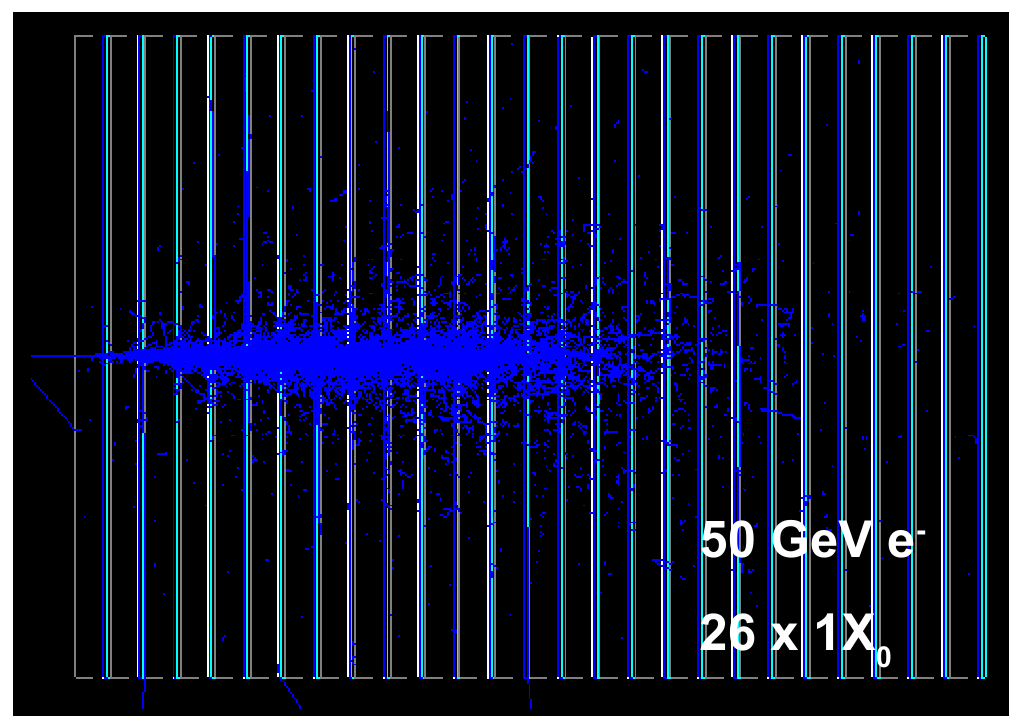
\includegraphics[width=\cmsFigWidth]{figures/e_50GeV_uniform_26x0.png}
    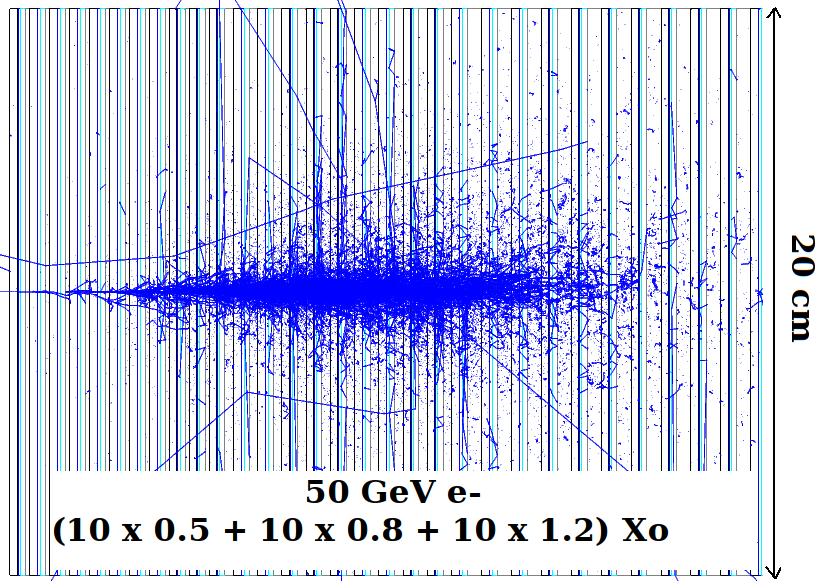
\includegraphics[width=\cmsFigWidth]{figures/e_50GeV_concept_v3.png}
    \caption{Event displays of a 50 GeV electron showers in the
      standalone simulation. Left: uniform 26 layers of 1 X$_0$
      each. Right: 30 layers in three blocks of different
      thicknesses. Electron deposits are shown in blue. Photons have
      been hidden for better visibility.}
    \label{fig:g4vis}
  \end{center}
\end{figure}

The simulation uses the QGSP\_FTFP\_BERT physics list, with the default cuts
for electrons, positrons and photons reduced to 10\,$\mu$m in the
silicon. The default elsewhere is 1\,mm. With 700\,$\mu$m in Si,
a 420 keV (5.8 keV) electron (photon) would deposit all its energy in
one step. With the reduced 10\,$\mu$m, the energy threshold is 32 keV
for electrons, and 990 eV for photons.


\subsubsection{Energy calibration and resolution}

Different methods are used to measure the total energy:
\begin{itemize}
\item raw energy: simply the sum of the energy deposited in Geant4 in
  the silicon in the full detector volume (30 layers of $20 \times
  20$\,cm$^2$).
\item weighted energy: sum of the energy deposited in the Si, but
  weighted differently according to which sampling section they belong
  to. Simplest weights are the ratio of sampling thicknesses in X$_0$,
  i.e. 1 for layers 0-9, 0.8/0.5 for layers 10-19 and 1.2/0.5 for
  layers 20-29. Weights can also be optimised to minimise the energy
  resolution for all energies.
\item Fit of the shower profile: allowing for example to recover the
  shower leakage for higher energies.
\end{itemize}

For the first two methods, the total energy is fitted, per incoming
energy generated, by a gaussian. The mean is used for calibration, and
the resolution is defined as the ratio of the width over the mean.

The calibration curve is shown in Figure~\ref{fig:eCalib} left, for
single electrons. Figure~\ref{fig:eCalib} right, shows the energy
resolution as a function of the incoming energy. For incoming energies
below 150 GeV, 2500 events have been generated, and 1250 above.

%@TODO replace with Pedro's plots with all 3 methods in.
\begin{figure}[h!]
  \begin{center}
    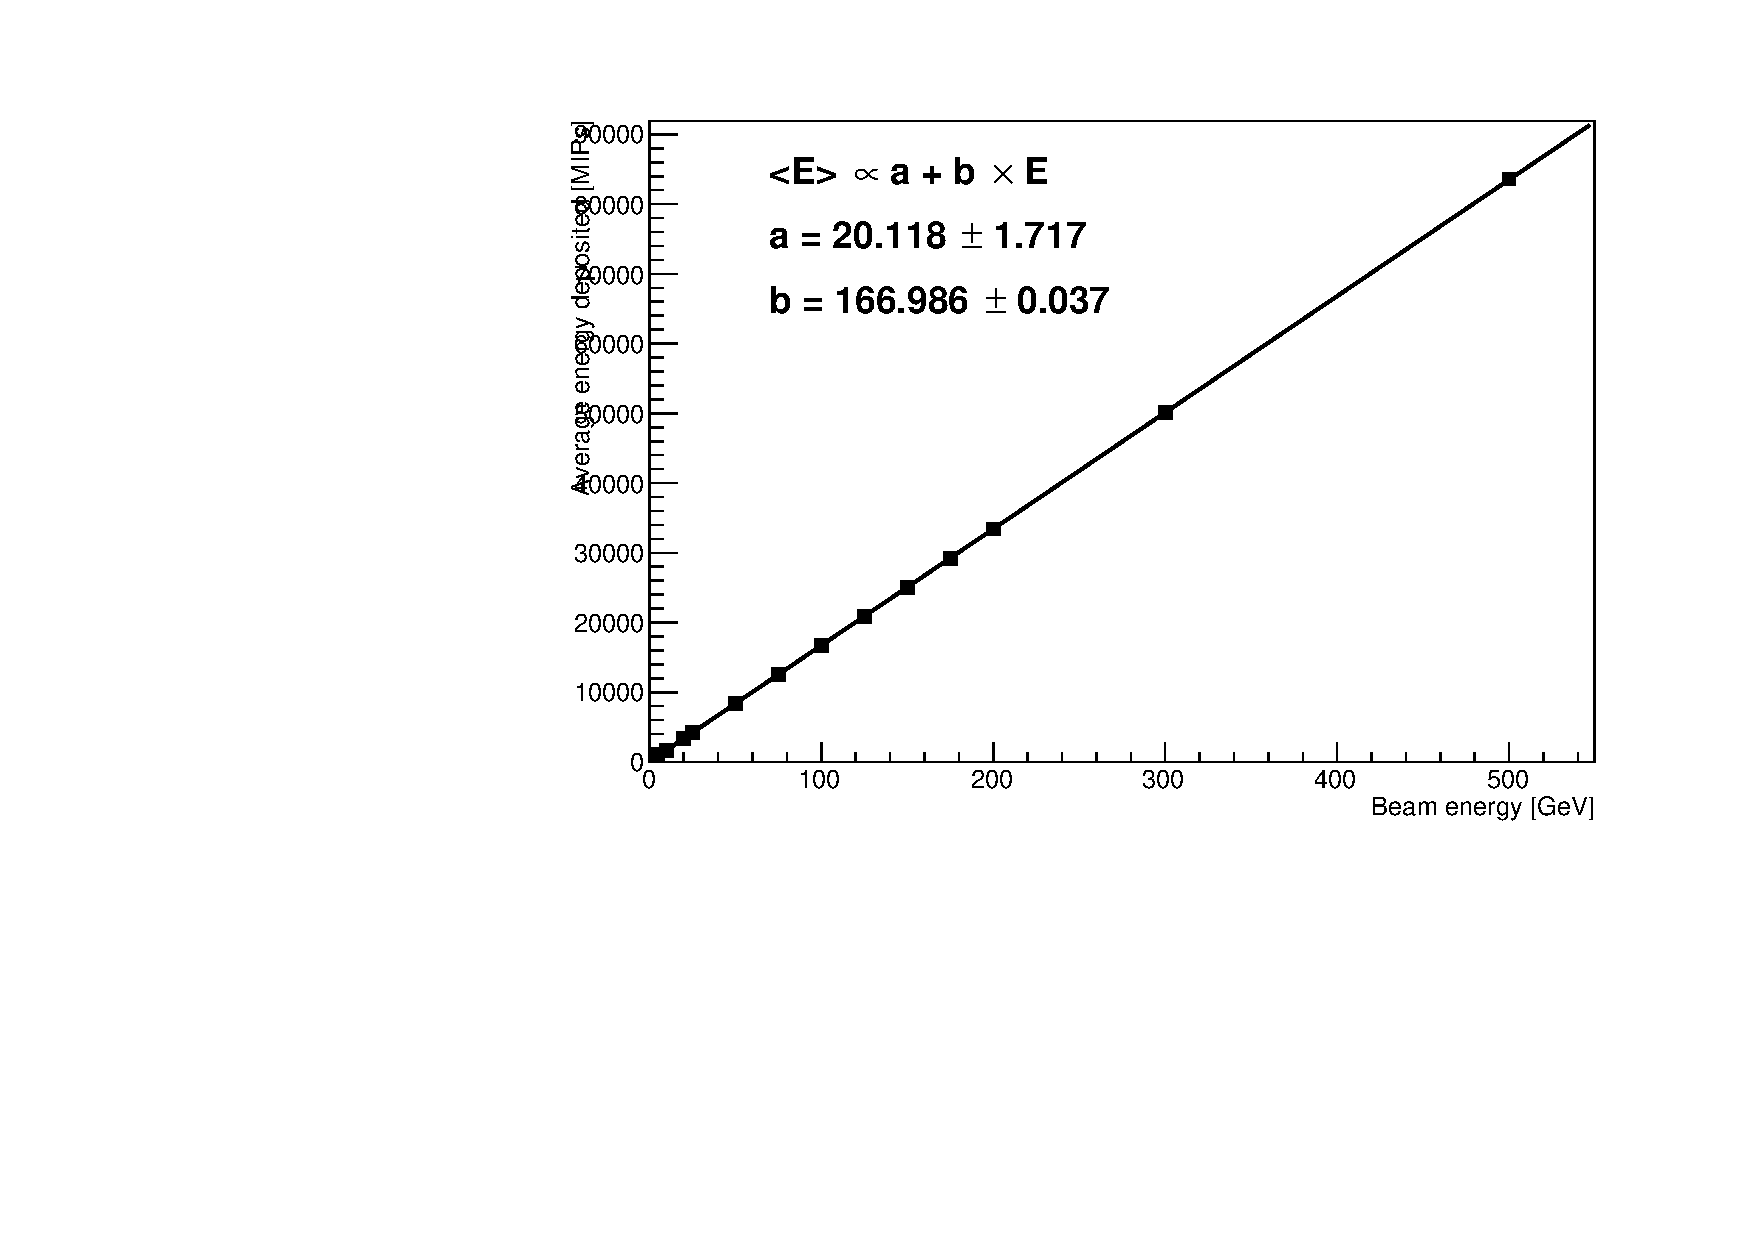
\includegraphics[width=\cmsFigWidth]{figures/e_calibFit.pdf}
    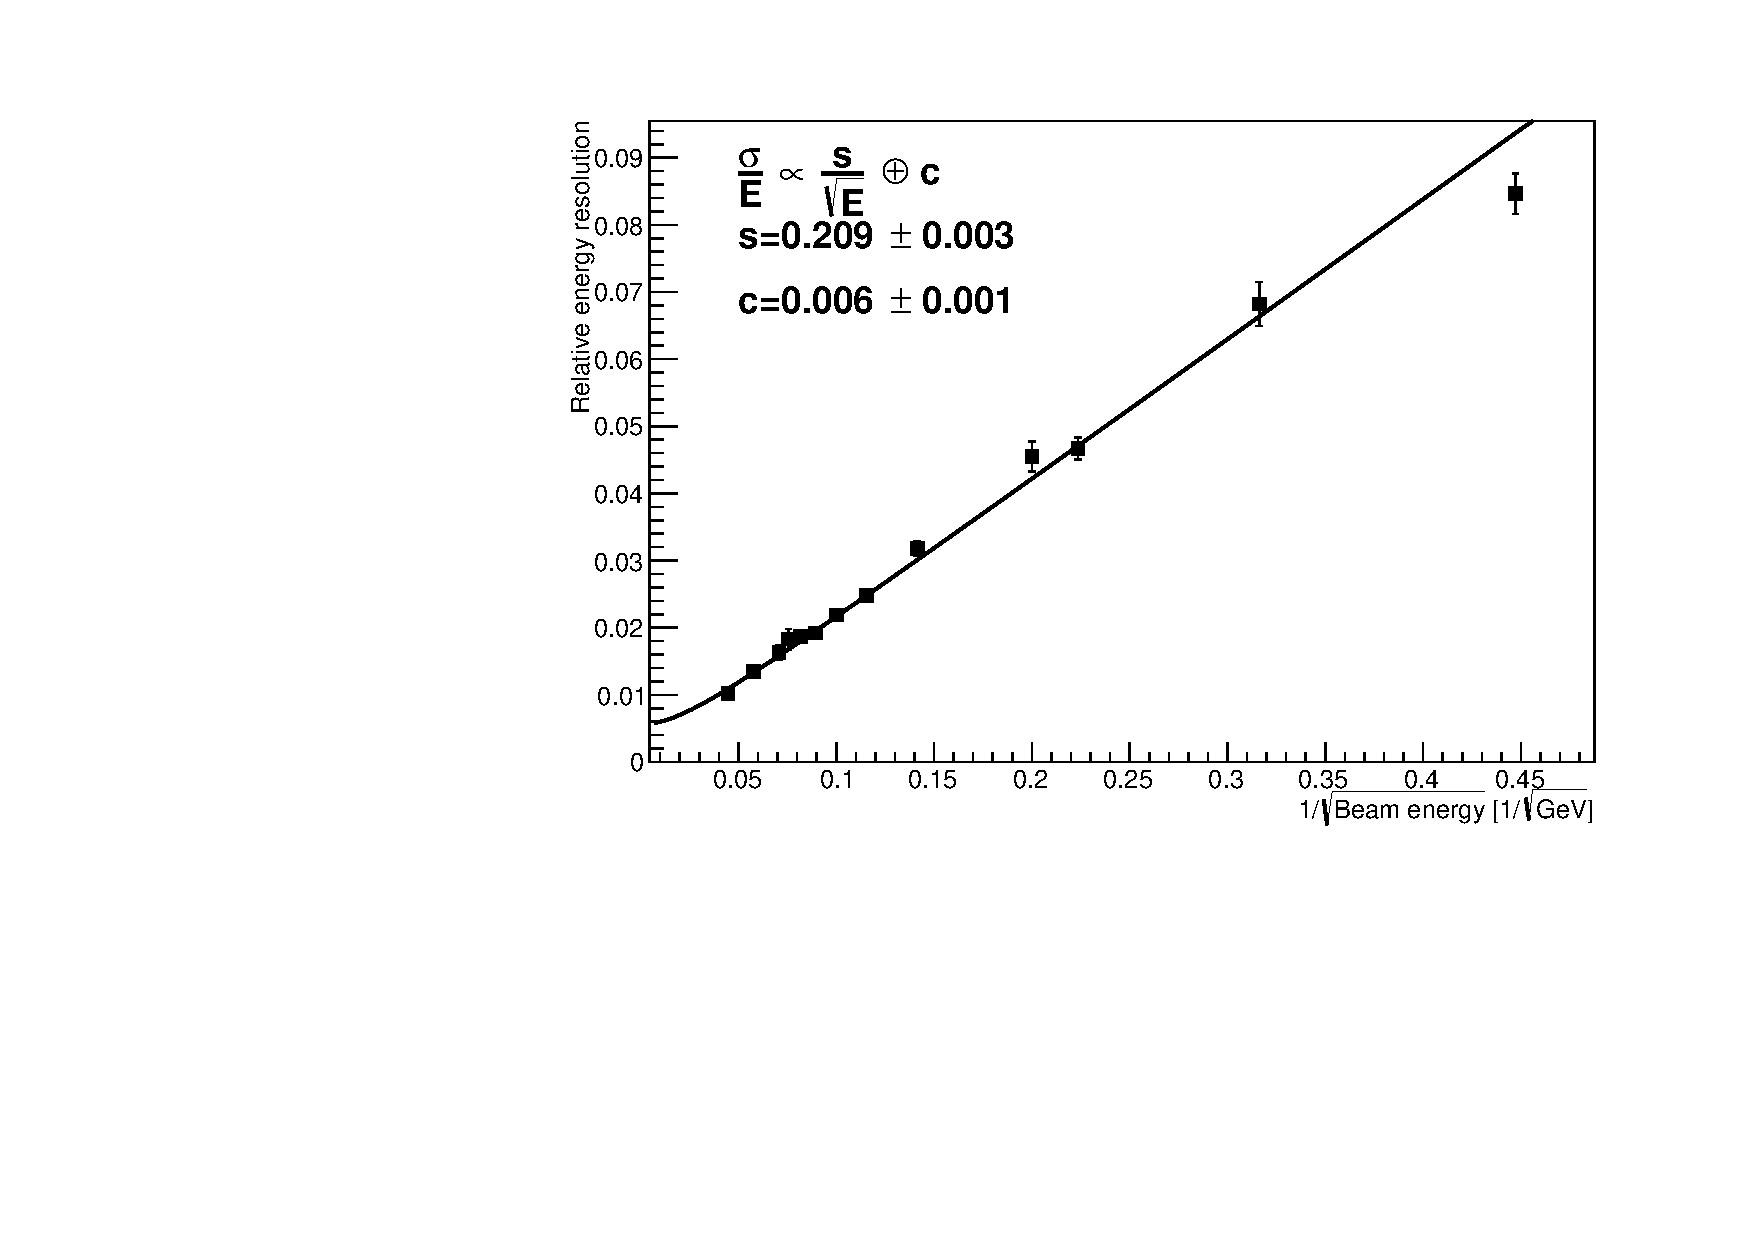
\includegraphics[width=\cmsFigWidth]{figures/e_resoFit.pdf}
    \caption{Reconstructed energy as a function of the generated
      energy E (left) and energy resolution as a function of
      $\frac{1}{\sqrt{E}}$ (right), for single electron events.}
    \label{fig:g4vis}
  \end{center}
\end{figure}



% Pedro
%
%
%
\clearpage
\section{Characterization of electromagnetic shower properties with
a Si-Pb sampling calorimeter}
\label{sec:emshowerproperties}

\FIXME{Add introduction}

%%
%%
%%
\subsection{Longitudinal evolution and energy estimation}
\label{subsec:longevol}

In order to characterize the longitudinal evolution of the showers in
our setup we count the total energy deposited by all hits in the Si layers. 
Energy is measured relatively to the estimated MIP signal (see details
ahead in Sec.~\ref{sec:digi}).
In this study electron events are used: for incoming energies
below 150\GeV, 2500 events have been generated; for higher energies
1250 events are used.

Figure~\ref{fig:showerfits} shows the longitudinal shower evolution
for single electron events as function of the \Xnot transversed in the
detector.
It can be observed that the level of energy fluctuations for low
energetic electrons is non-negligible, with $\delta$ deposits
dominating the contribution to the total energy deposited in each Si
layer.
For sufficiently energetic electrons these contributions become of
second order and the characterization of the shower is dominated by
the statistical fluctuations in the number of particles comprising the shower.
For very high energy showers ($>$150\GeV) part of the energy can't be
contained in the detector setup using 25\Xnot. Given that in this
regime the showers are dominated by statistical fluctuations in its
composition a fit to the longitudinal profile can be used safely and
used to estimate the leakage fraction.

\begin{figure}[h!]
  \begin{center}
    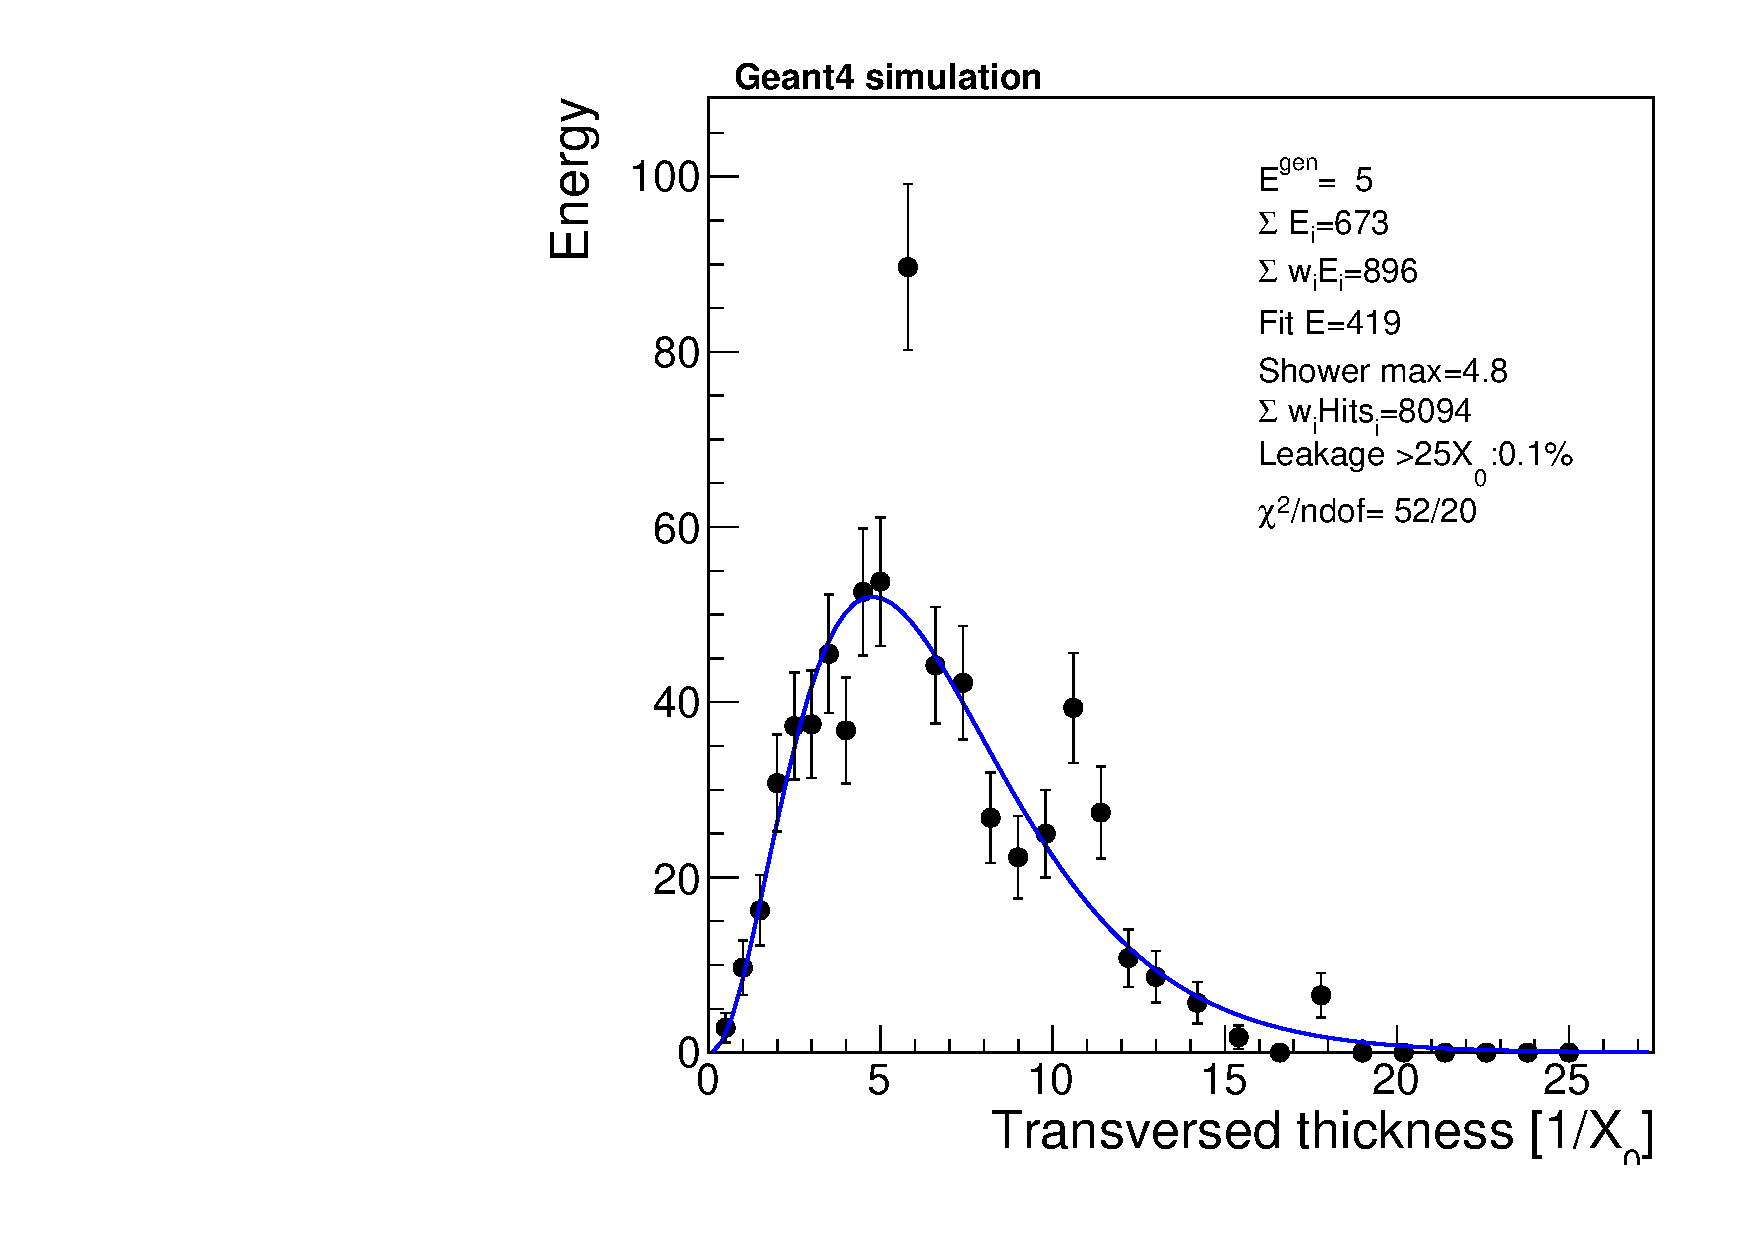
\includegraphics[width=0.24\textwidth]{figures/version_3e_5_5_showerfits}
    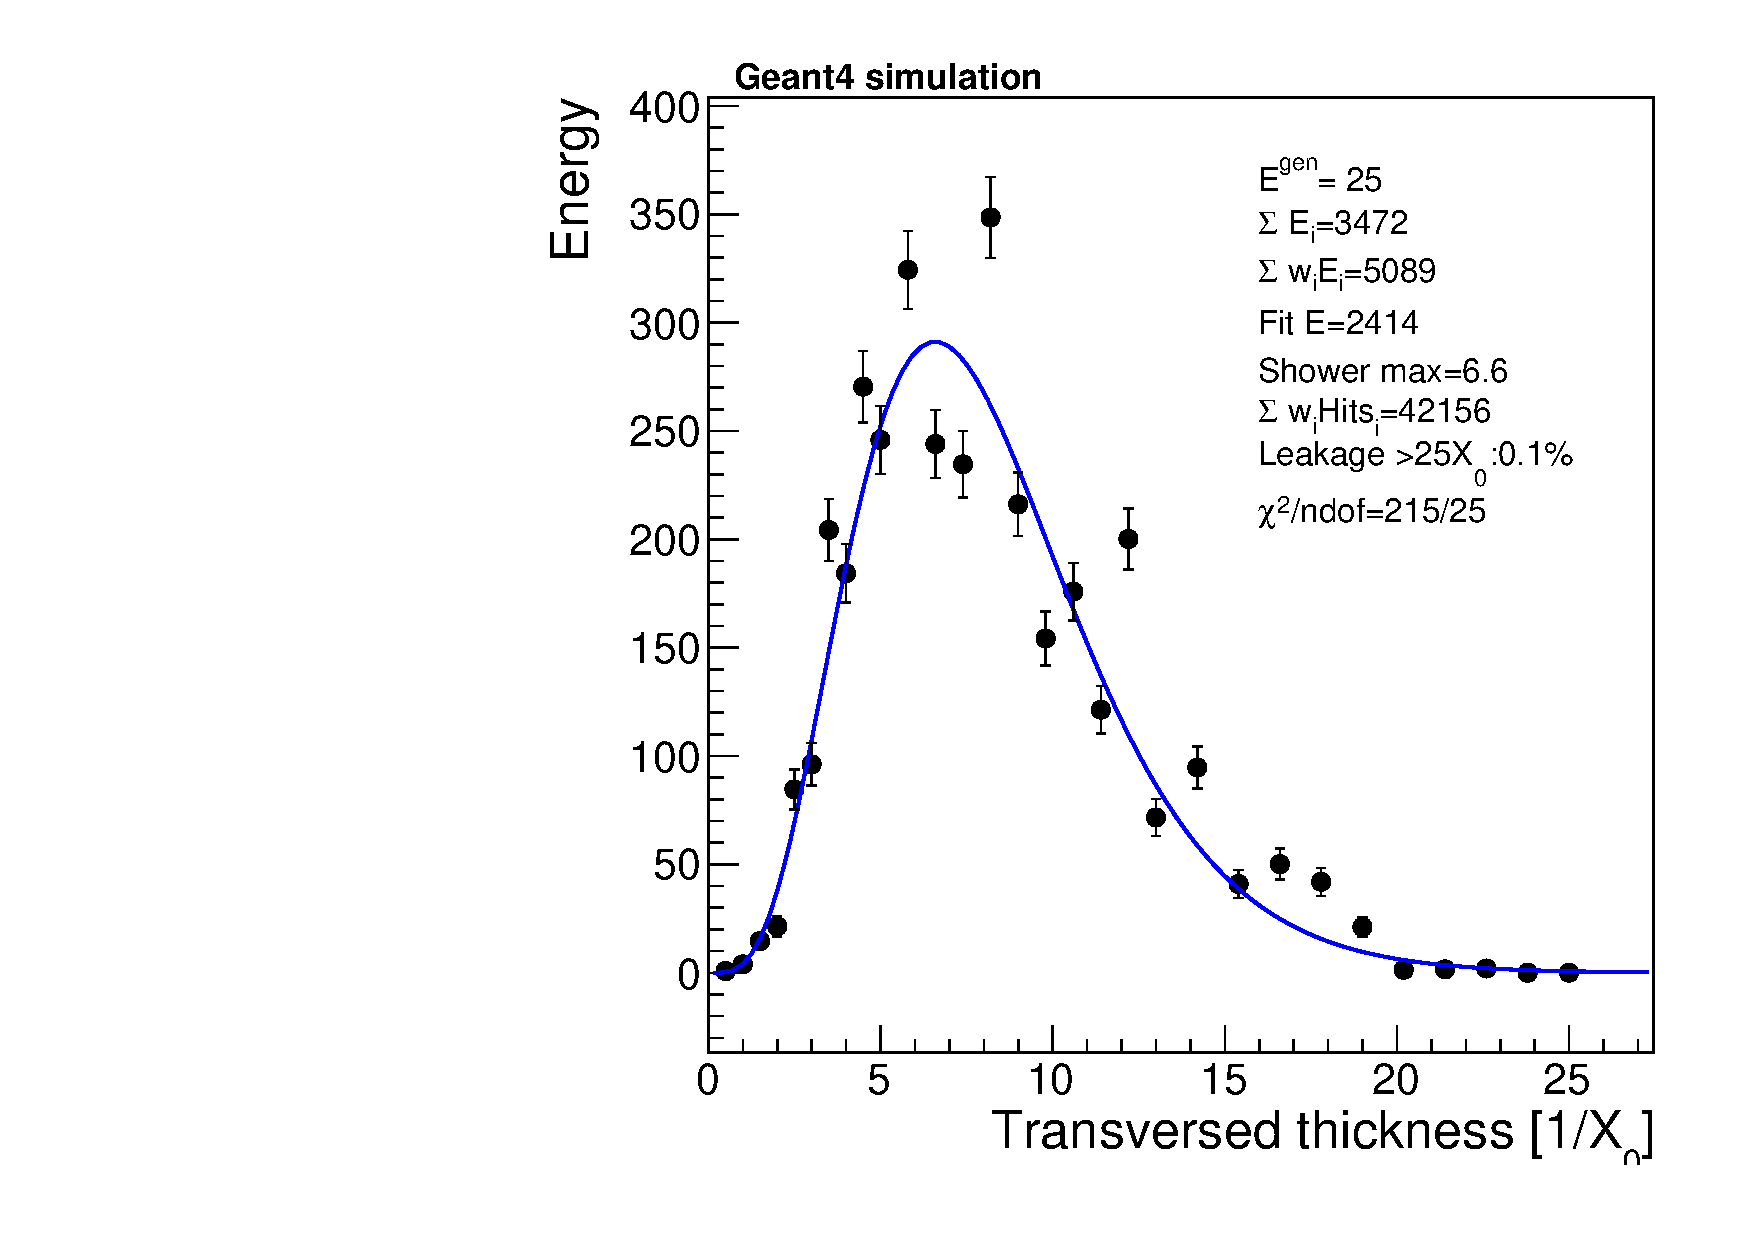
\includegraphics[width=0.24\textwidth]{figures/version_3e_25_8_showerfits}
    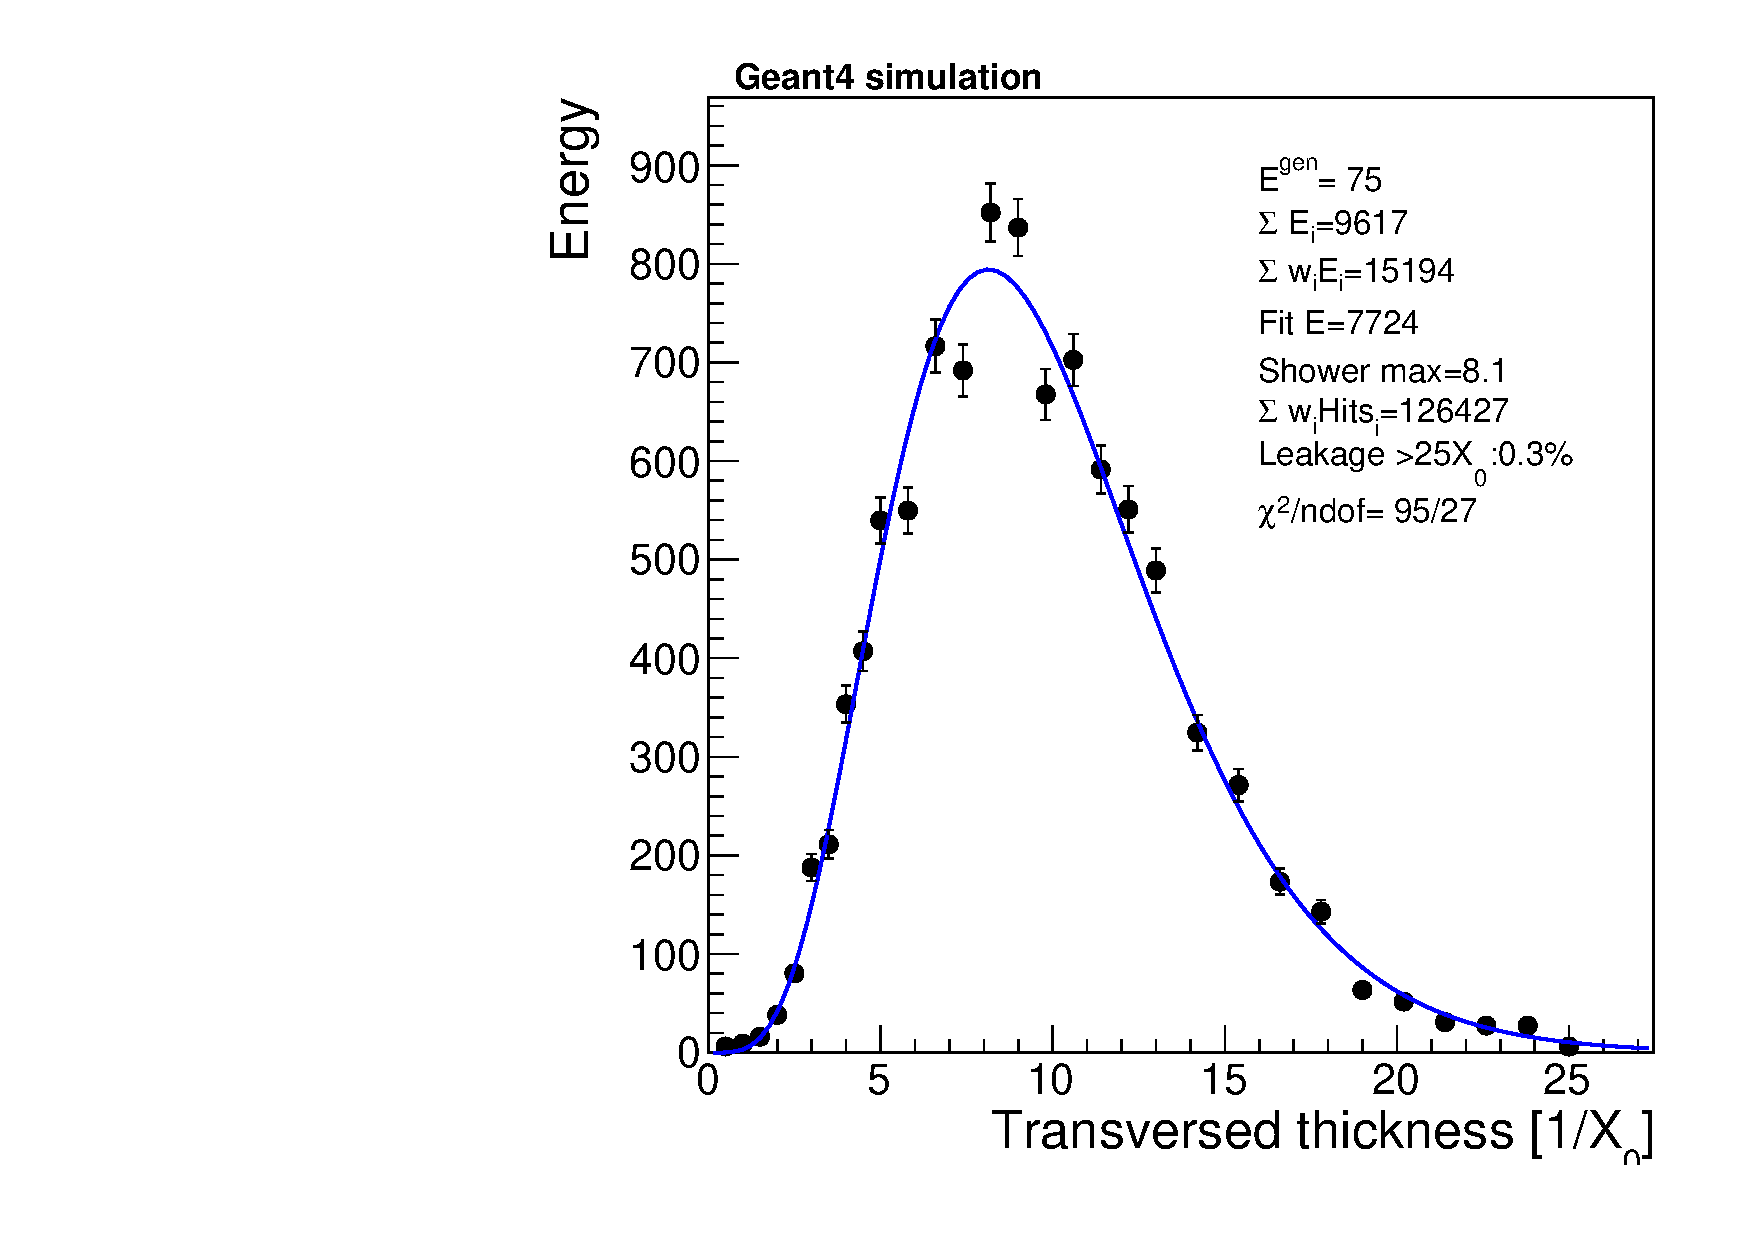
\includegraphics[width=0.24\textwidth]{figures/version_3e_75_6_showerfits}
    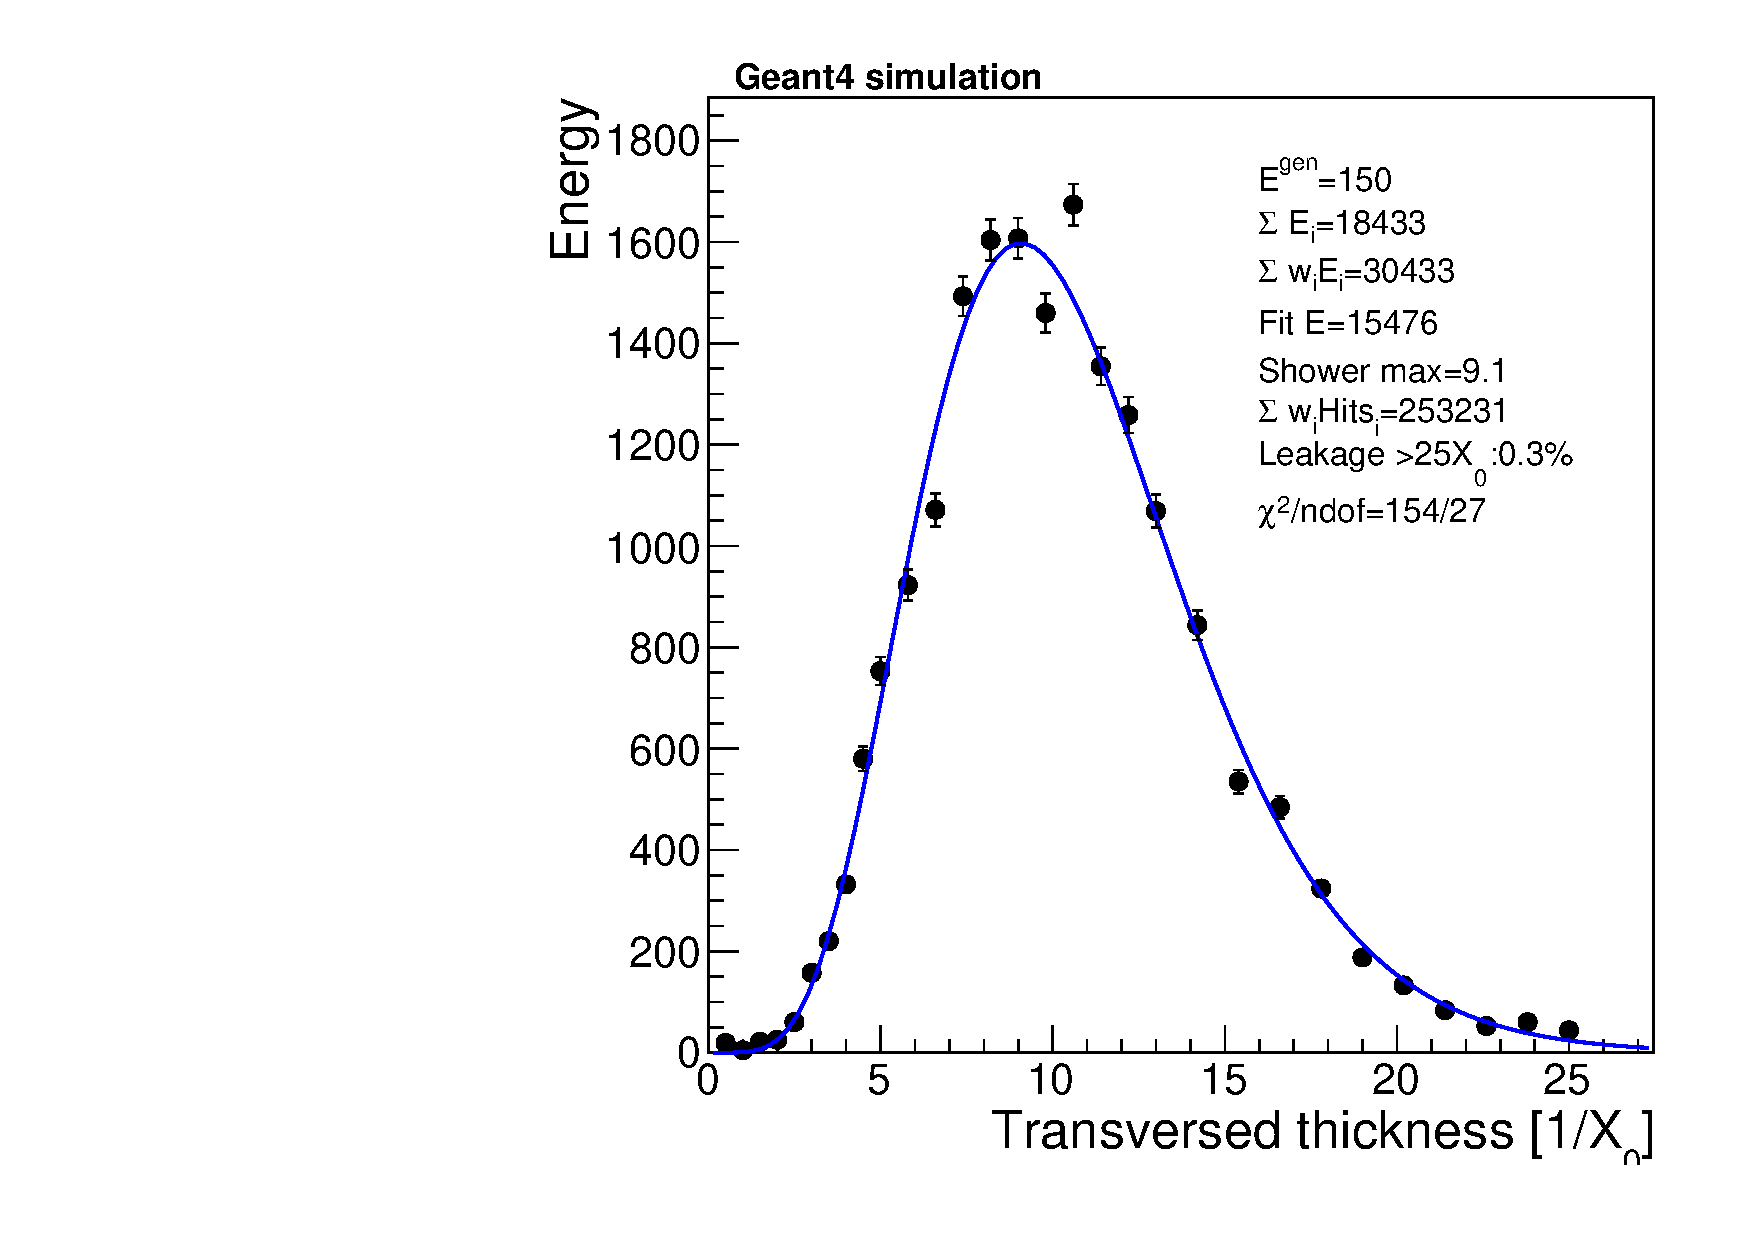
\includegraphics[width=0.24\textwidth]{figures/version_3e_150_6_showerfits}
    \caption{From {\em left} to {\em right}: energy deposits in different Si layers for single
      electron events with energies: 10, 25, 50, 100\GeV. The deposits
    are shown as function of the transversed distance in \Xnot
    units. A fit is overlaid using the functional form described in
    the text. 
     The results obtained for the different energy estimators
     considered in the analysis, as well as for the shower leakage
     estimated from the fit, are shown in the caption}
    \label{fig:showerfits}
  \end{center}
\end{figure}

Thus, different methods to estimate the total energy of the shower are
compared:

\begin{description}

\item[Raw energy] we sum inclusively of all the energy deposited in
  the Si layers assuming the full sensitive area volume;

\item[Weighted energy] we sum the energy deposited in each Si layer
  normalized by the material overburden of the sampling section,\ie:

\begin{equation}
{\rm weighted~E}=\sum_{i=1}^{N} \frac{X_0^i}{X_0^1}\cdot E_i
\label{eq:weightenest}
\end{equation}

For the baseline setup these weights correspond to 1 for section A,
1.6 for section B and 2.4 for section B.
These weights can also be optimised to minimise the energy resolution
for the incoming energy range of interest.

\item[Shower profile fit] - a functional form is used to adjust the
  measured energy deposits in each layer:

\begin{equation}
\mathcal{E}(x)=\alpha\cdot x^{a} \cdot e^{-bx} 
\label{eq:showerprof}
\end{equation}

where x is the transversed material overburden measured in \Xnot
units. This approach is expected to recover the shower leakage for
higher incident energies.

\item[Shower maximum] - the position of the shower max can be used as a
  coarse estimator for the energy. It can be estimated after the
  shower fit by the ratio $X_{0}^{\max}=b/a$.

\item[Hit counting] - this estimator, altough impossible to be used in
  reality, is used to gauge to potential of the setup. We use the
  weighted sum  of the number of hits generated per Si layer as an
  estimator of the initial energy. The weights are the same as define
  in Eq.~\ref{eq:weightenest}.

\end{description}

For each method the distribution of the estimator is fitted with a
gaussian for each incoming generated beam energy. An unbinned-likelihood fit is
used for this purpose. Figures~\ref{fig:fithitcount}
and~\ref{fig:fitwen}
show two examples using the weighted energy and the hit counting
estimators correspondingly.

\begin{figure}[h!]
  \begin{center}
    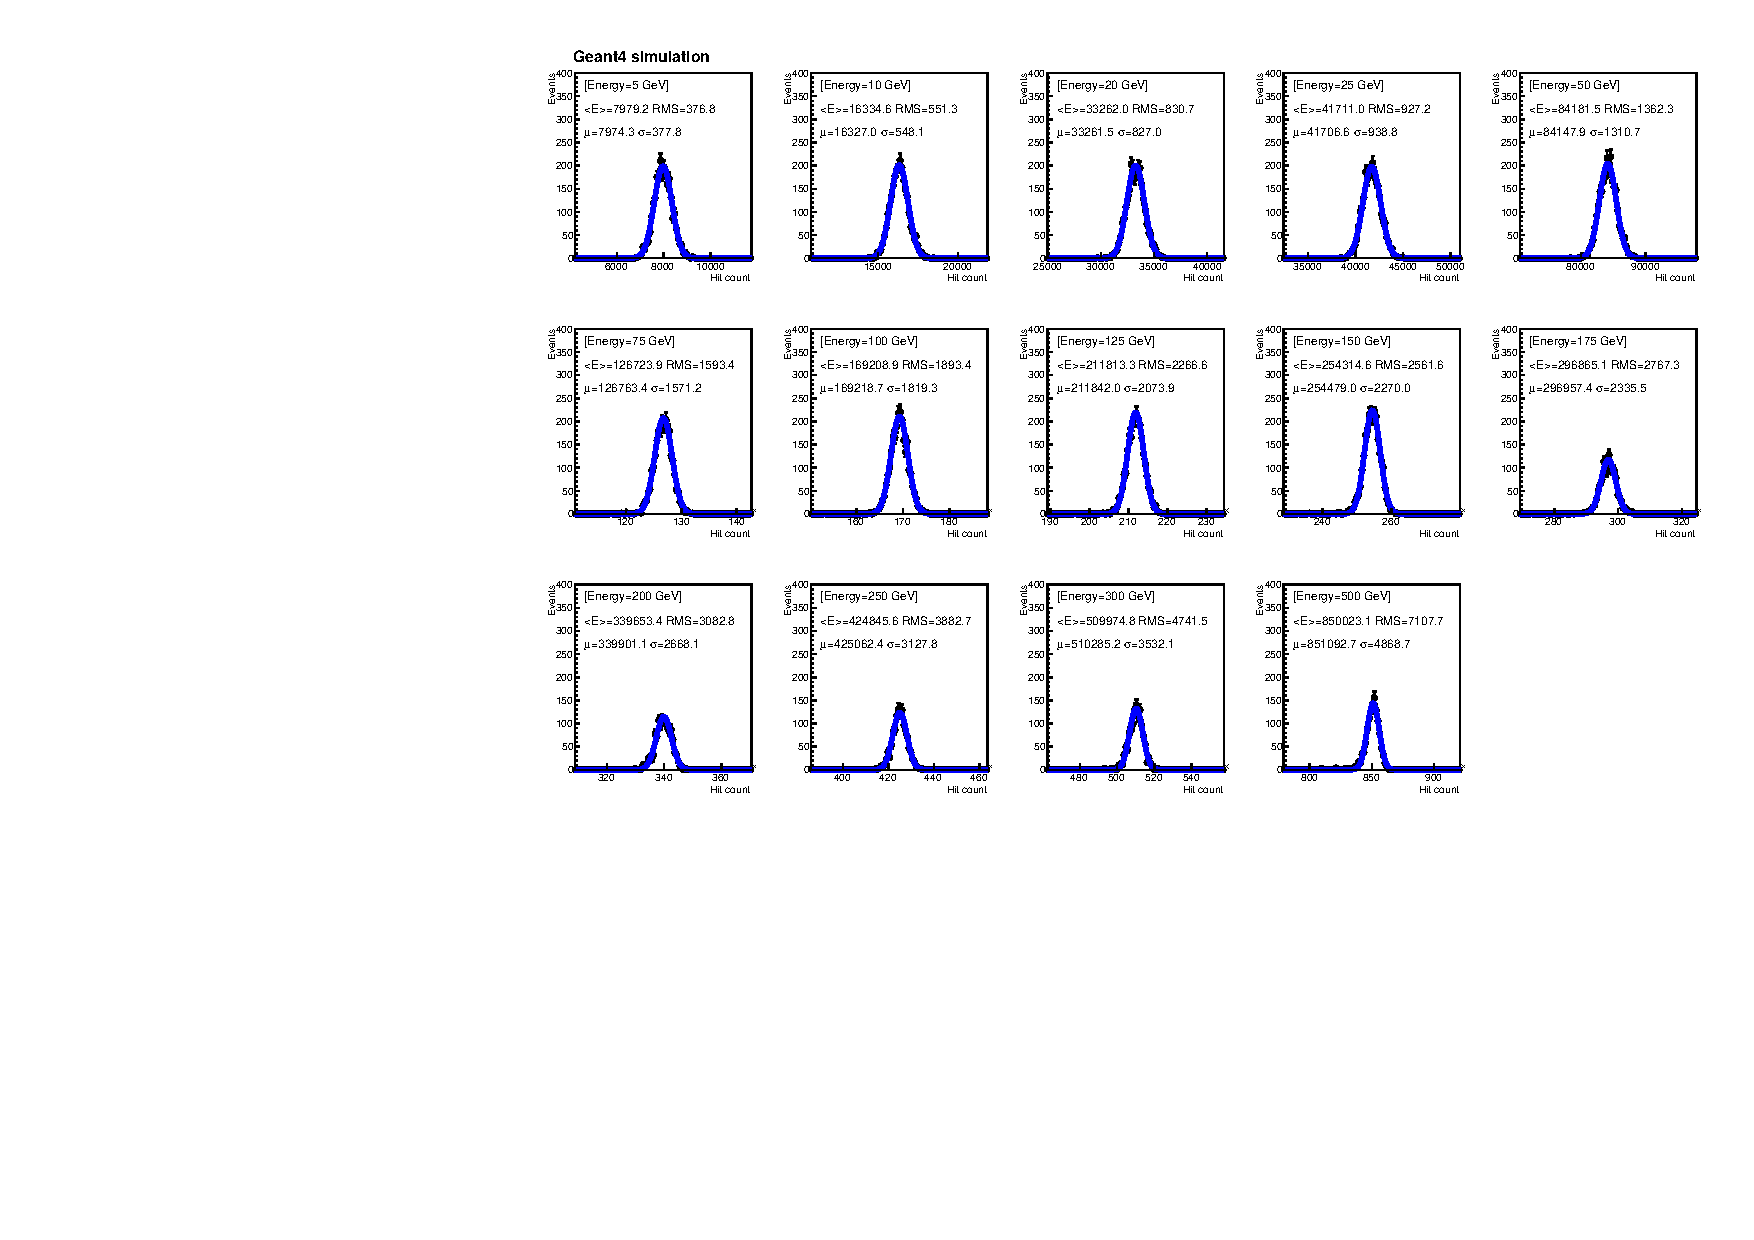
\includegraphics[width=0.99\textwidth]{figures/recenergy_nemHits}
    \caption{Weighted energy sum estimator distributions for different
    beam energies. The result of an unbinned-likelihood fit of a gaussian is
    superimposed. The mean and average of the distribution and the
    gaussian are compared in the caption.}
    \label{fig:fithitcount}
  \end{center}
\end{figure}

\begin{figure}[h!]
  \begin{center}
    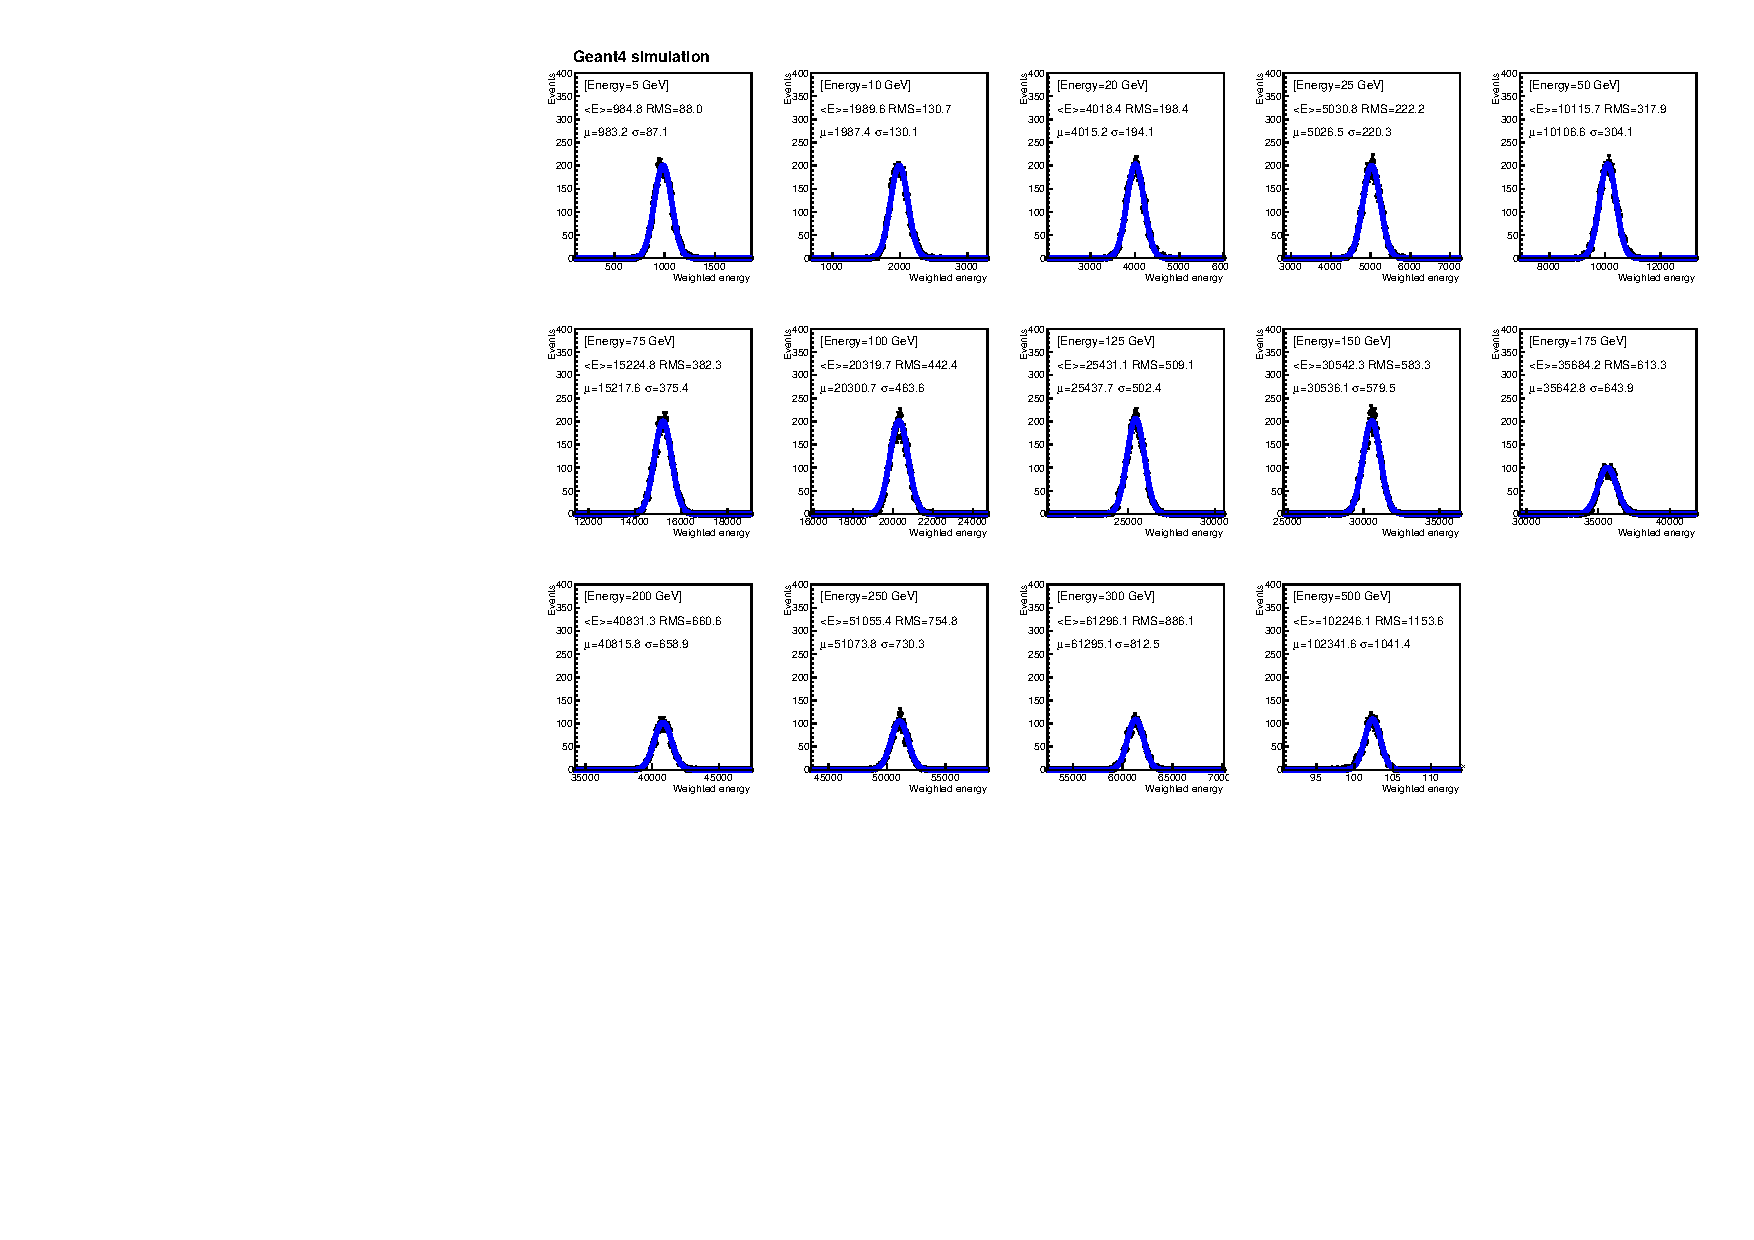
\includegraphics[width=0.99\textwidth]{figures/recenergy_sumWEn}
    \caption{Similar to Fig.~\ref{fig:fithitcount} for the weighted energy sum estimator.}
    \label{fig:fitwen}
  \end{center}
\end{figure}

The parameters of the fitted gaussians can be used for two purposes:
the mean is used to obtain the calibration (\ie dependency of the
energy estimator on the incoming energy) and the ratio of the width
with respect to the mean as an estimator for the resolution.
The calibration curves obtained are shown in Fig.~\ref{fig:baselinelinandresol}
{\em left} where linear behaviour is observed for all the estimators.
Figure~\ref{fig:baselinelinandresol} {\em right} shows the energy
resolution as a function of the incoming energy. 
A fit to a resolution model is super-imposed for each curve. The
resolution model is based on the quadratic sum of a stochastic term
(proportional to $1/\sqrt{E}$) with a constant term,\ie:

\begin{equation}
\left(\frac{\sigma_{\rm E}}{\rm E}\right)^2 = \left(\frac{\sigma_{\rm
      stoch}}{\sqrt{\rm E}}\right)^2+\sigma_{\rm cte}^2
\label{eq:resmodel}
\end{equation}

As expected, altough the raw energy estimator scales faster with
energy (\ie has smaller stochastic term) its resolution fastly
saturates at a non-negligible due to the fact that the sampling is
non-uniform. The weighted energy estimator is able to recover from
this attaining a baseline resolution of the order of 20.9\%. The
residual constant term can be almost fully removed with a shower
leakage recovery algorithm such as the one provided by the fitted
energy estimator - in this approach the constant term is observed to
be compatible with 0.
The hit count approach yields the best resolution expected to be
attainable with this setup. The shower max estimator has worse
resolution and large constant term.

\begin{figure}[h!]
  \begin{center}
   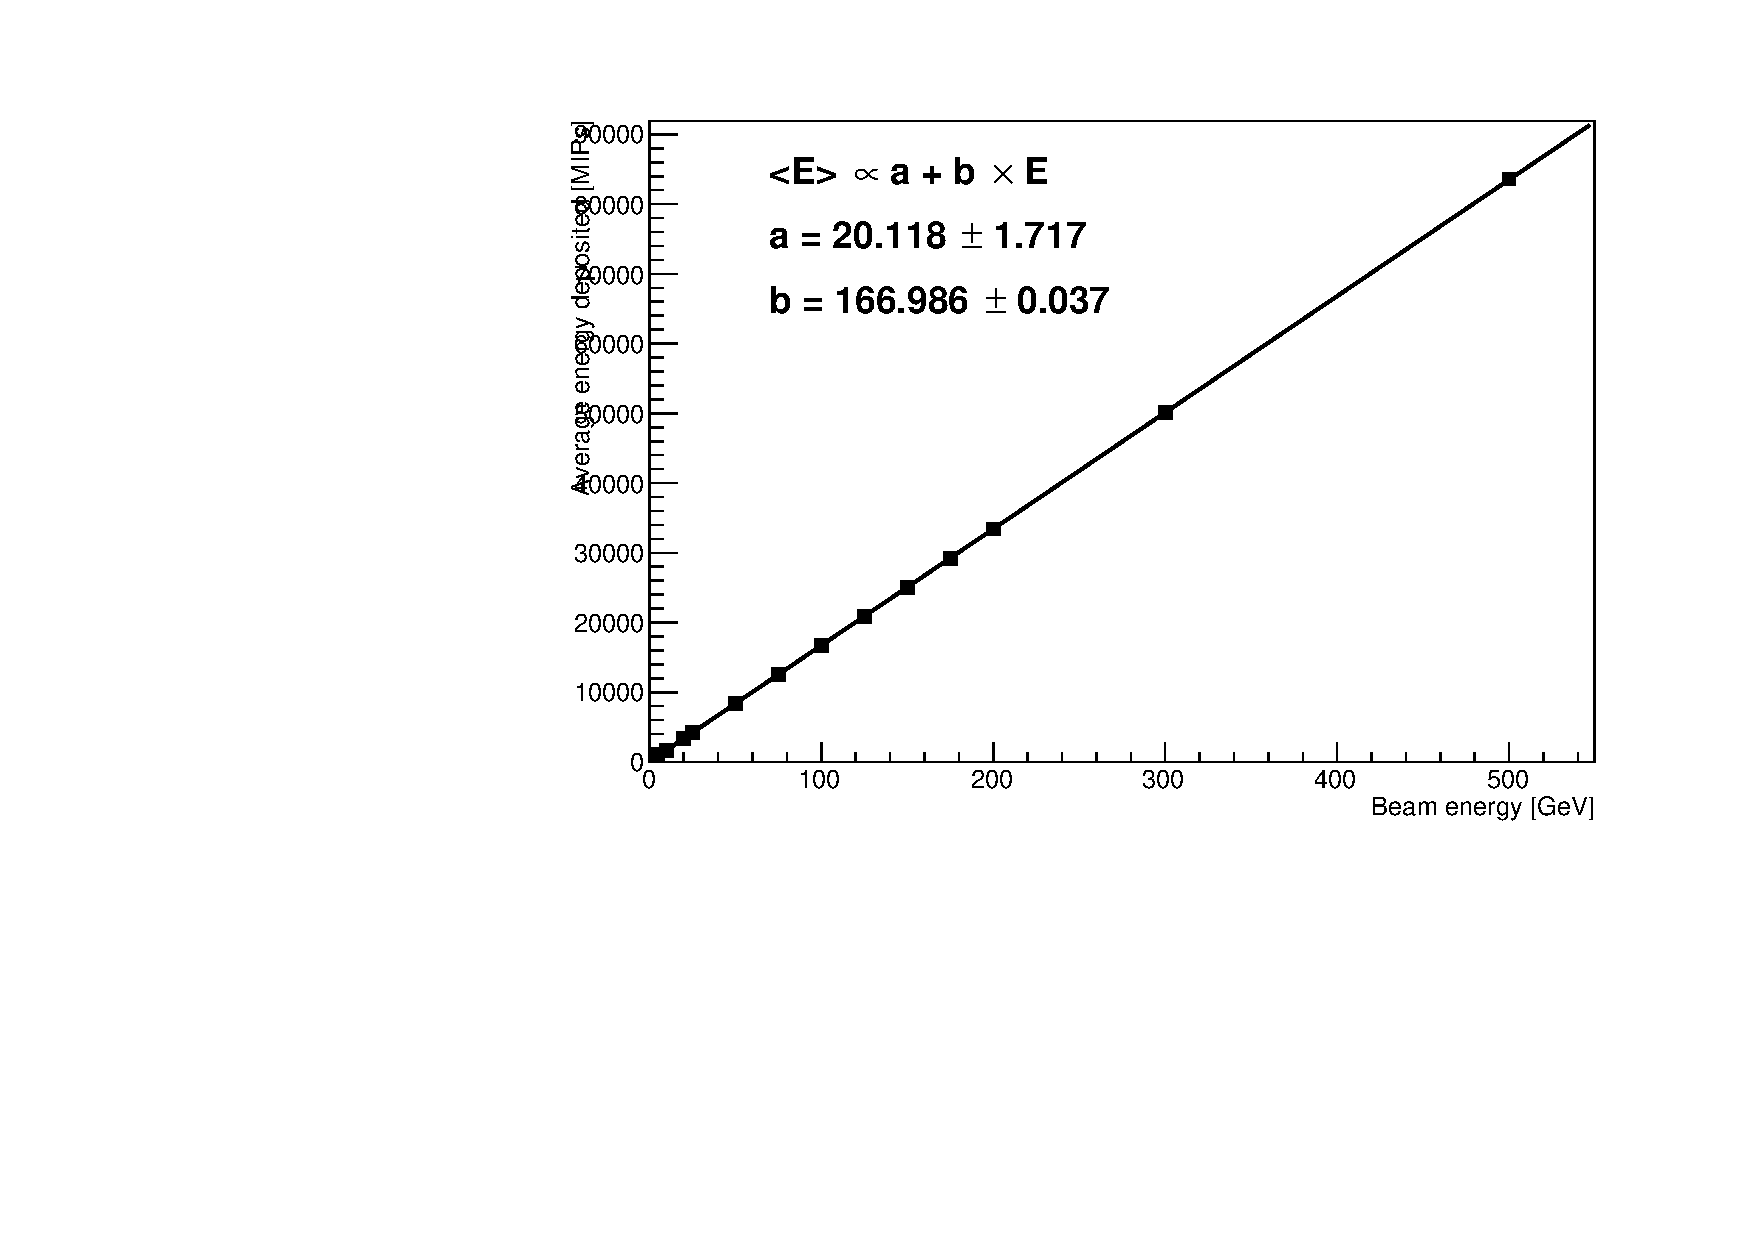
\includegraphics[width=0.48\textwidth]{figures/e_calibFit}
    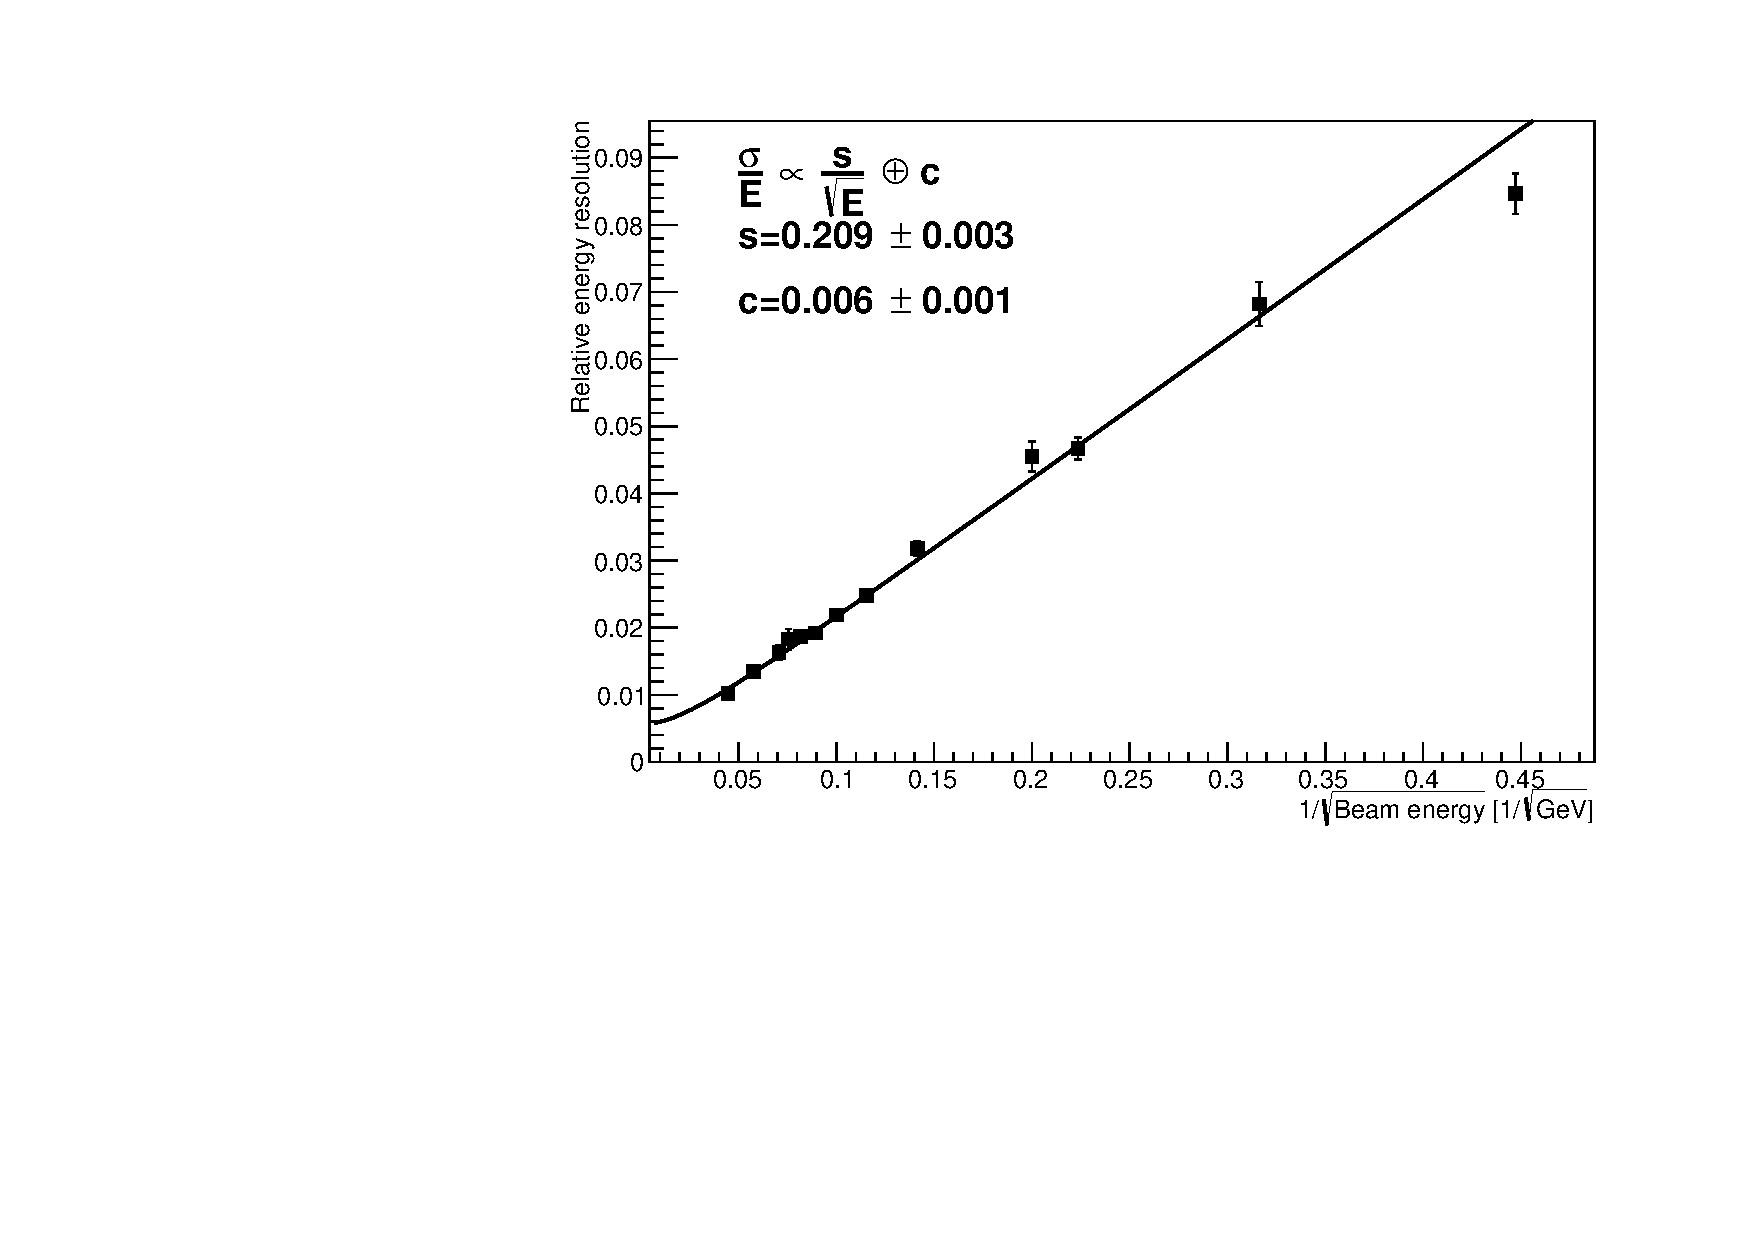
\includegraphics[width=0.48\textwidth]{figures/e_resoFit}
    \caption{{\em Left}: reconstructed energy (in MIP units) as a function of the generated
      energy E. {\em Right}: energy resolution as a function of
      $\frac{1}{\sqrt{E}}$. In both cases single electron events are simulated.}
    \label{fig:baselinelinandresol}
  \end{center}
\end{figure}

Figure~\ref{fig:longprofiles} summarizes the average energy profile
(and energy fluctuation) of the showers for different incident
energies.
The plot on the {\em left} is shown as function of the transversed
thickness transversed in the detector.
It can be observed that for incident energies below 5\GeV the shower
maximum will occur in average in the first section of the detector.
For energies up to 500\GeV the shower maximum will be contained in the
second section of the detector.
As explained above, the fitted longitudinal shower profile to each
event can be used as the estimator of the shower maximum. This
estimator can be used to re-map the energy deposits as function of the
distance to the shower maximum yielding the so-called centered shower
profile shown at the {\em center} of the figure.
This depicts the scaling property of the energy generated by shower
which yields the linear behaviour of the energy estimators used above.
The centered shower profile can be furthermore used to profile the
average fluctuations. This is shown on the {\em right}.
The core of the shower is, has expected, less prone to statistical
fluctuations with an intrinsic resolution of $\approx$10-15\% for
$E>50\GeV$.
The initial stage is prone to the largest fluctuations and the fine
sampling at these earlier stages may therefore provide additional handle on the energy
resolution. This will be discussed later in Section~\ref{sec:optim}.
The last part of the shower, as it will be shown next, is expected to
be dominated by the halo of the shower and, again, is prone to larger
statistical fluctuations with respect to the central region.

\begin{figure}[h!]
  \begin{center}
   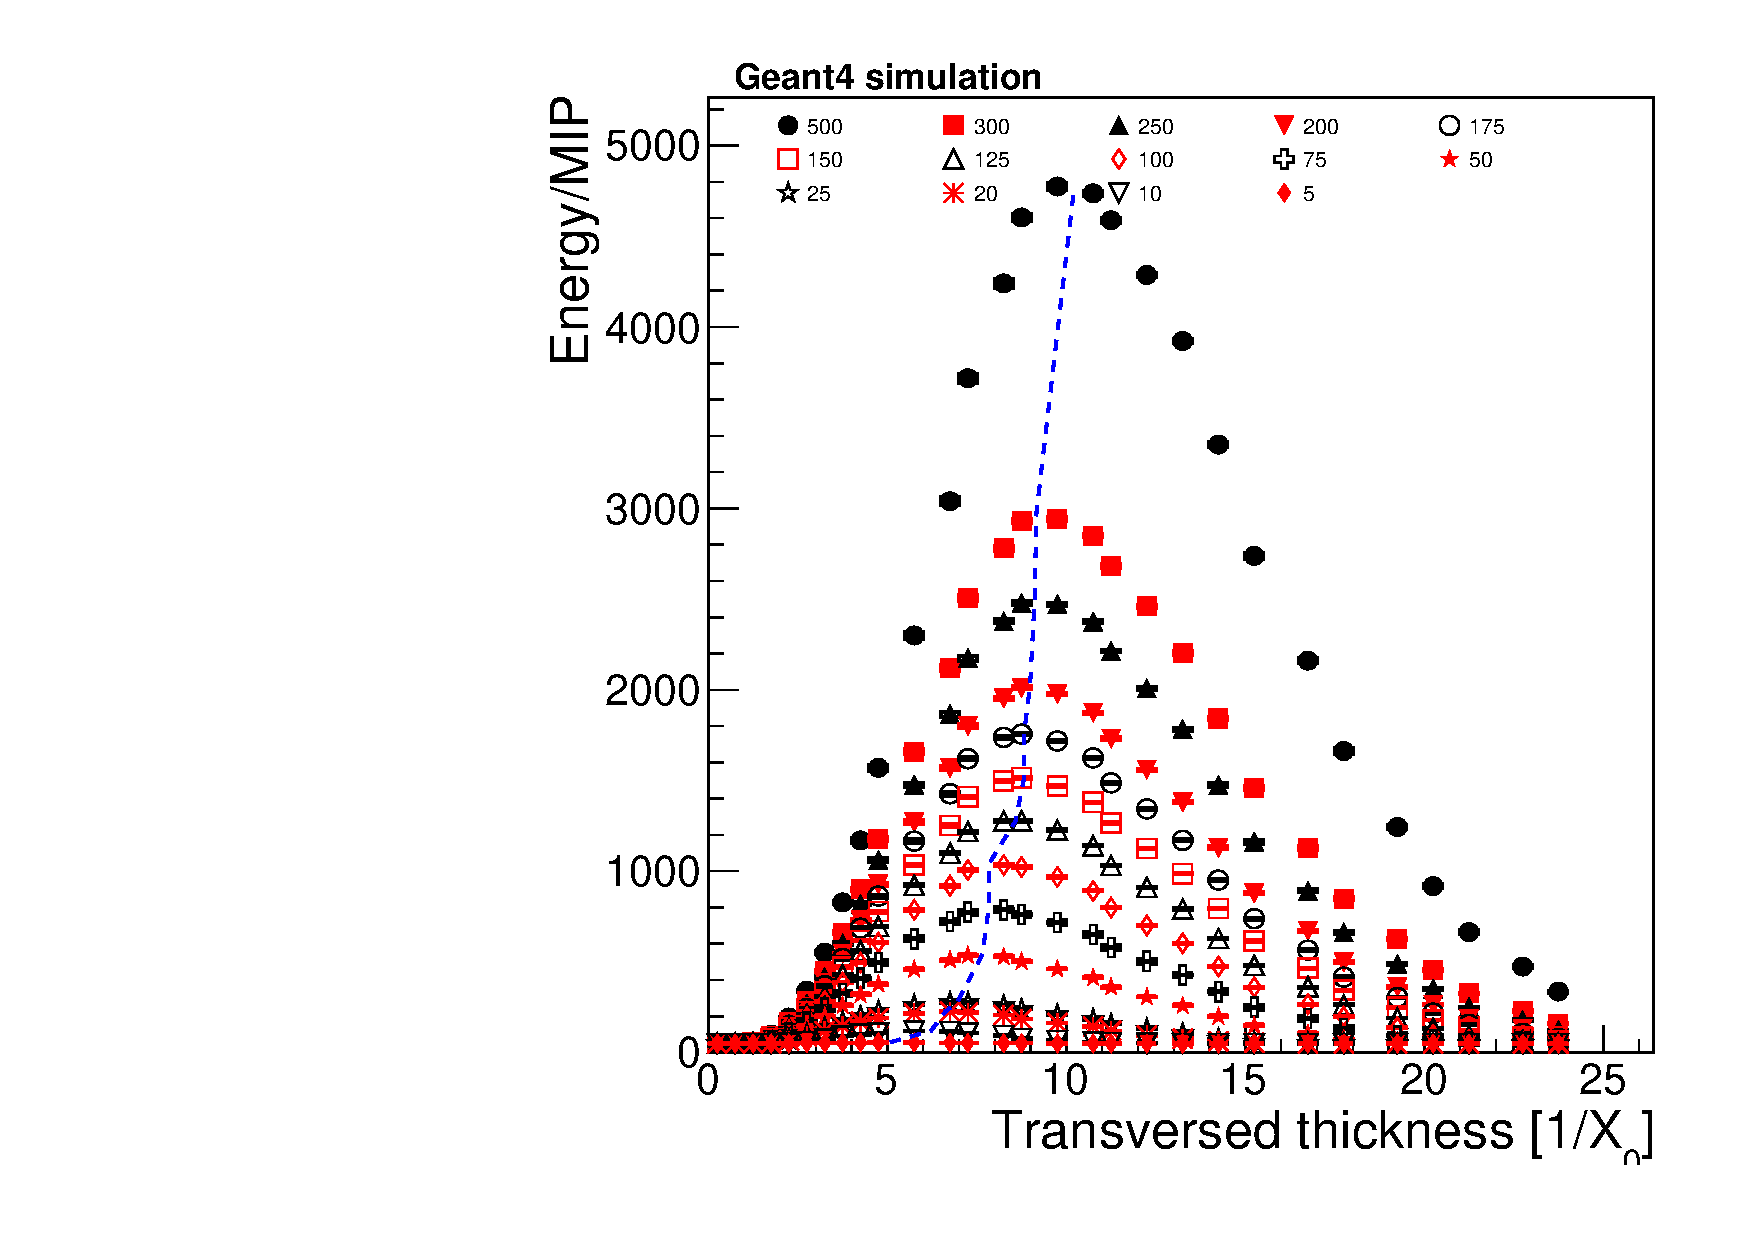
\includegraphics[width=0.32\textwidth]{figures/version_3_rawprof}
    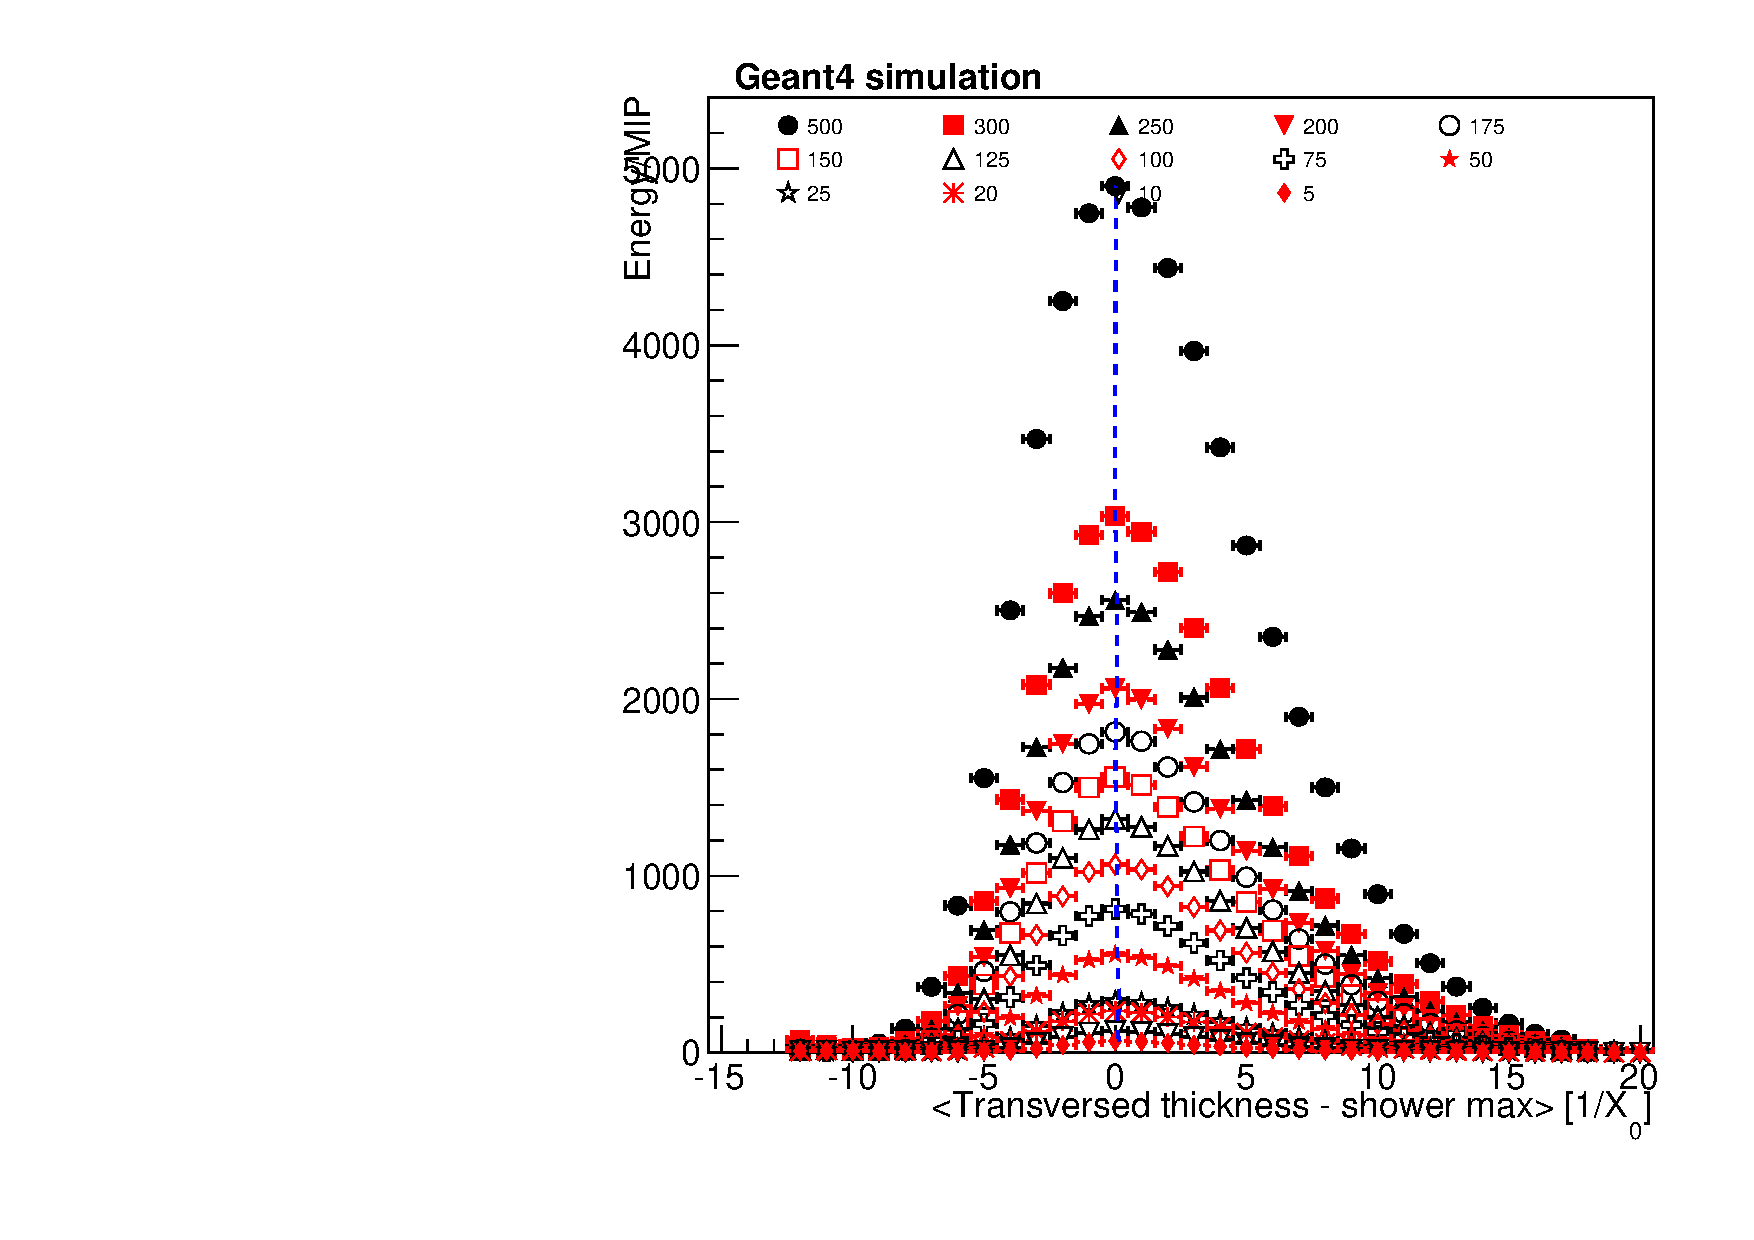
\includegraphics[width=0.32\textwidth]{figures/version_3_cenprof}
    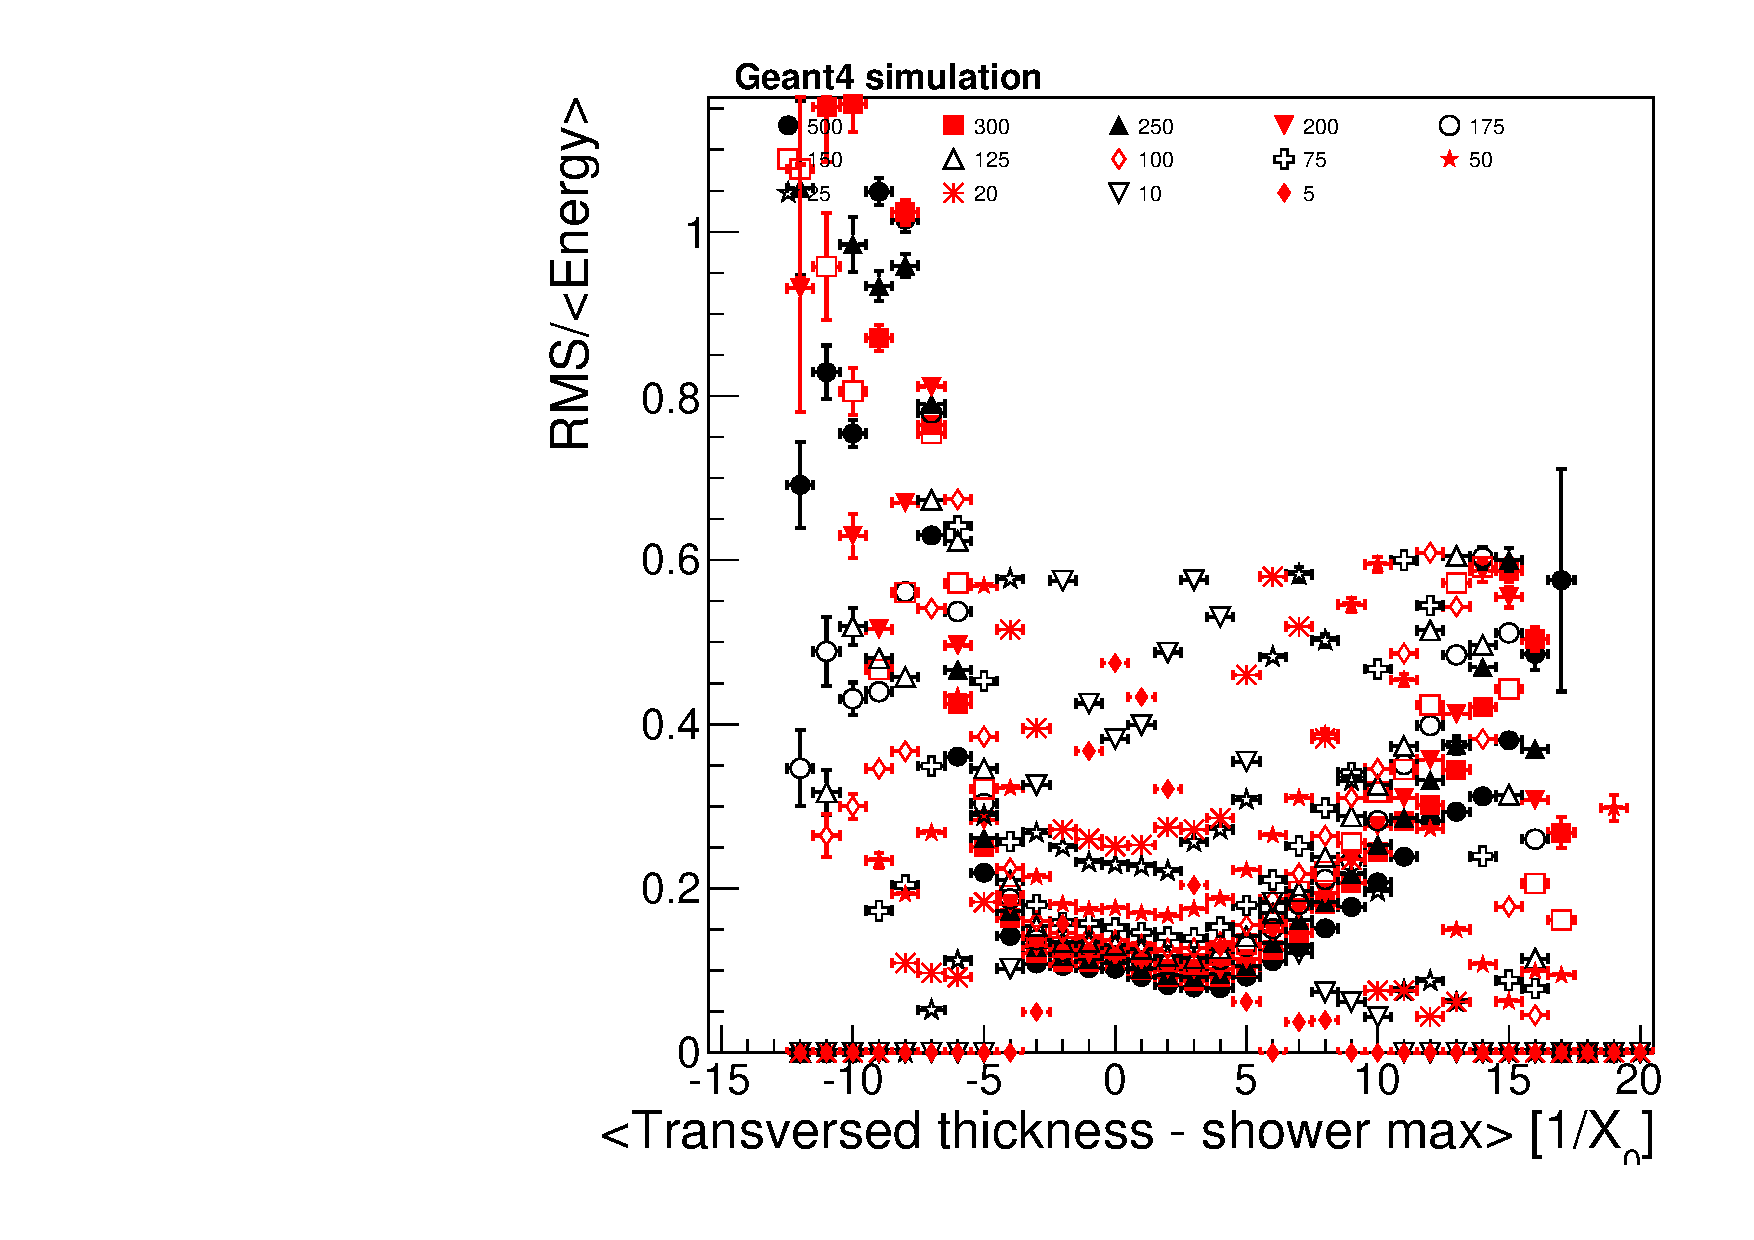
\includegraphics[width=0.32\textwidth]{figures/version_3_crelunc}
    \caption{{\em Left}: average energy deposited as function of the
      transversed thickness in the calorimeter. A blue curve connects
      the estimated shower maximum.
     {\em Center}: average energy deposited as function of the distance
     to the shower maximum estimated on an event-per-event basis.
    {\em Right}: average relative width of the energy deposits as
    function of the distance to the shower maximum estimated on an event-per-event basis.
   }
    \label{fig:longprofiles}
  \end{center}
\end{figure}

%%
%%
%%
\subsection{Transverse shower evolution and shower containment}
\label{subsec:transvevol}

\FIXME{Describe transverse shower properties and Moliere radius}

% Pedro
%
%
%
\clearpage
\section{Optimisation of the design}
\label{sec:optim}

\FIXME{Add introduction}

\FIXME{Varying the Silicon width test}

\FIXME{Varying the sampling fractions test}

\FIXME{Varying the absorber material test}



\begin{figure}[h!]
  \begin{center}
  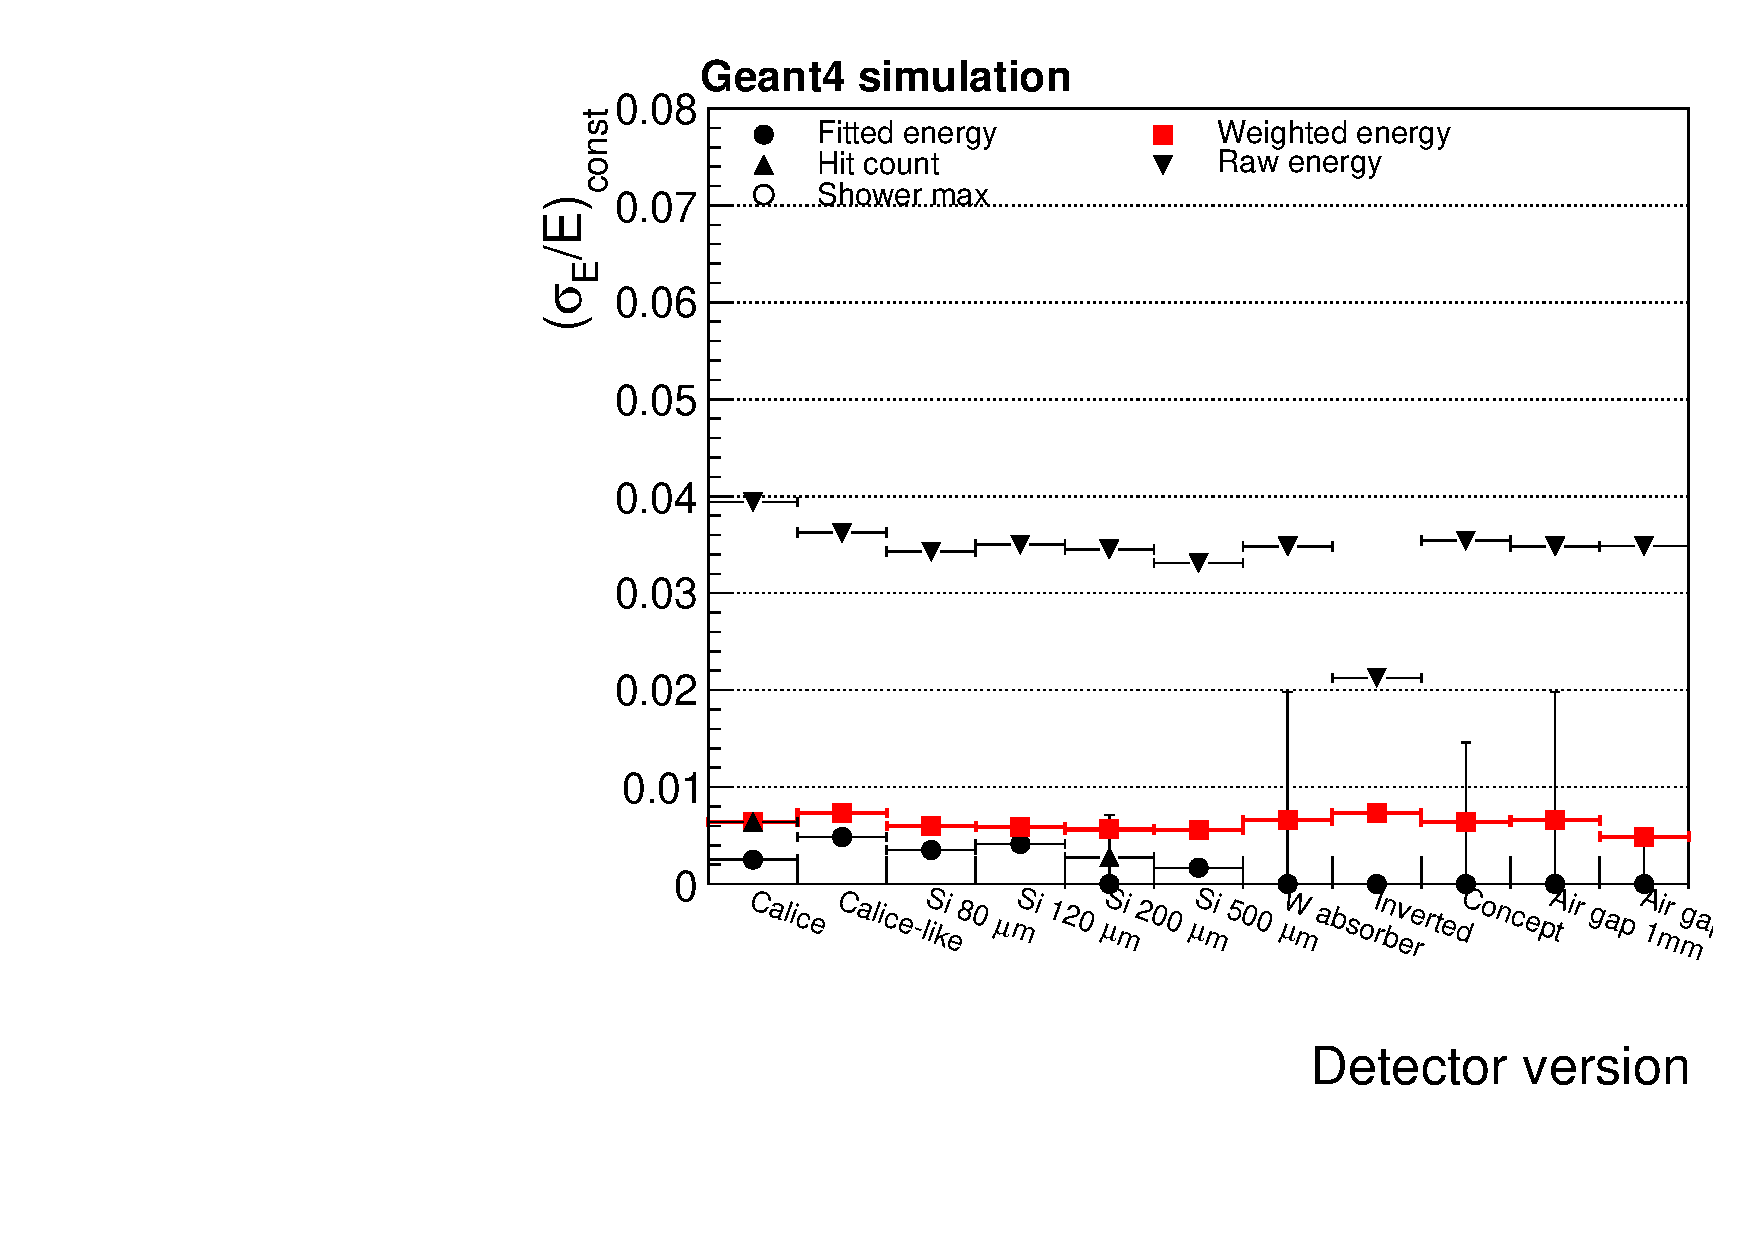
\includegraphics[width=0.75\textwidth]{figures/ResolutionSummary_const}\\
  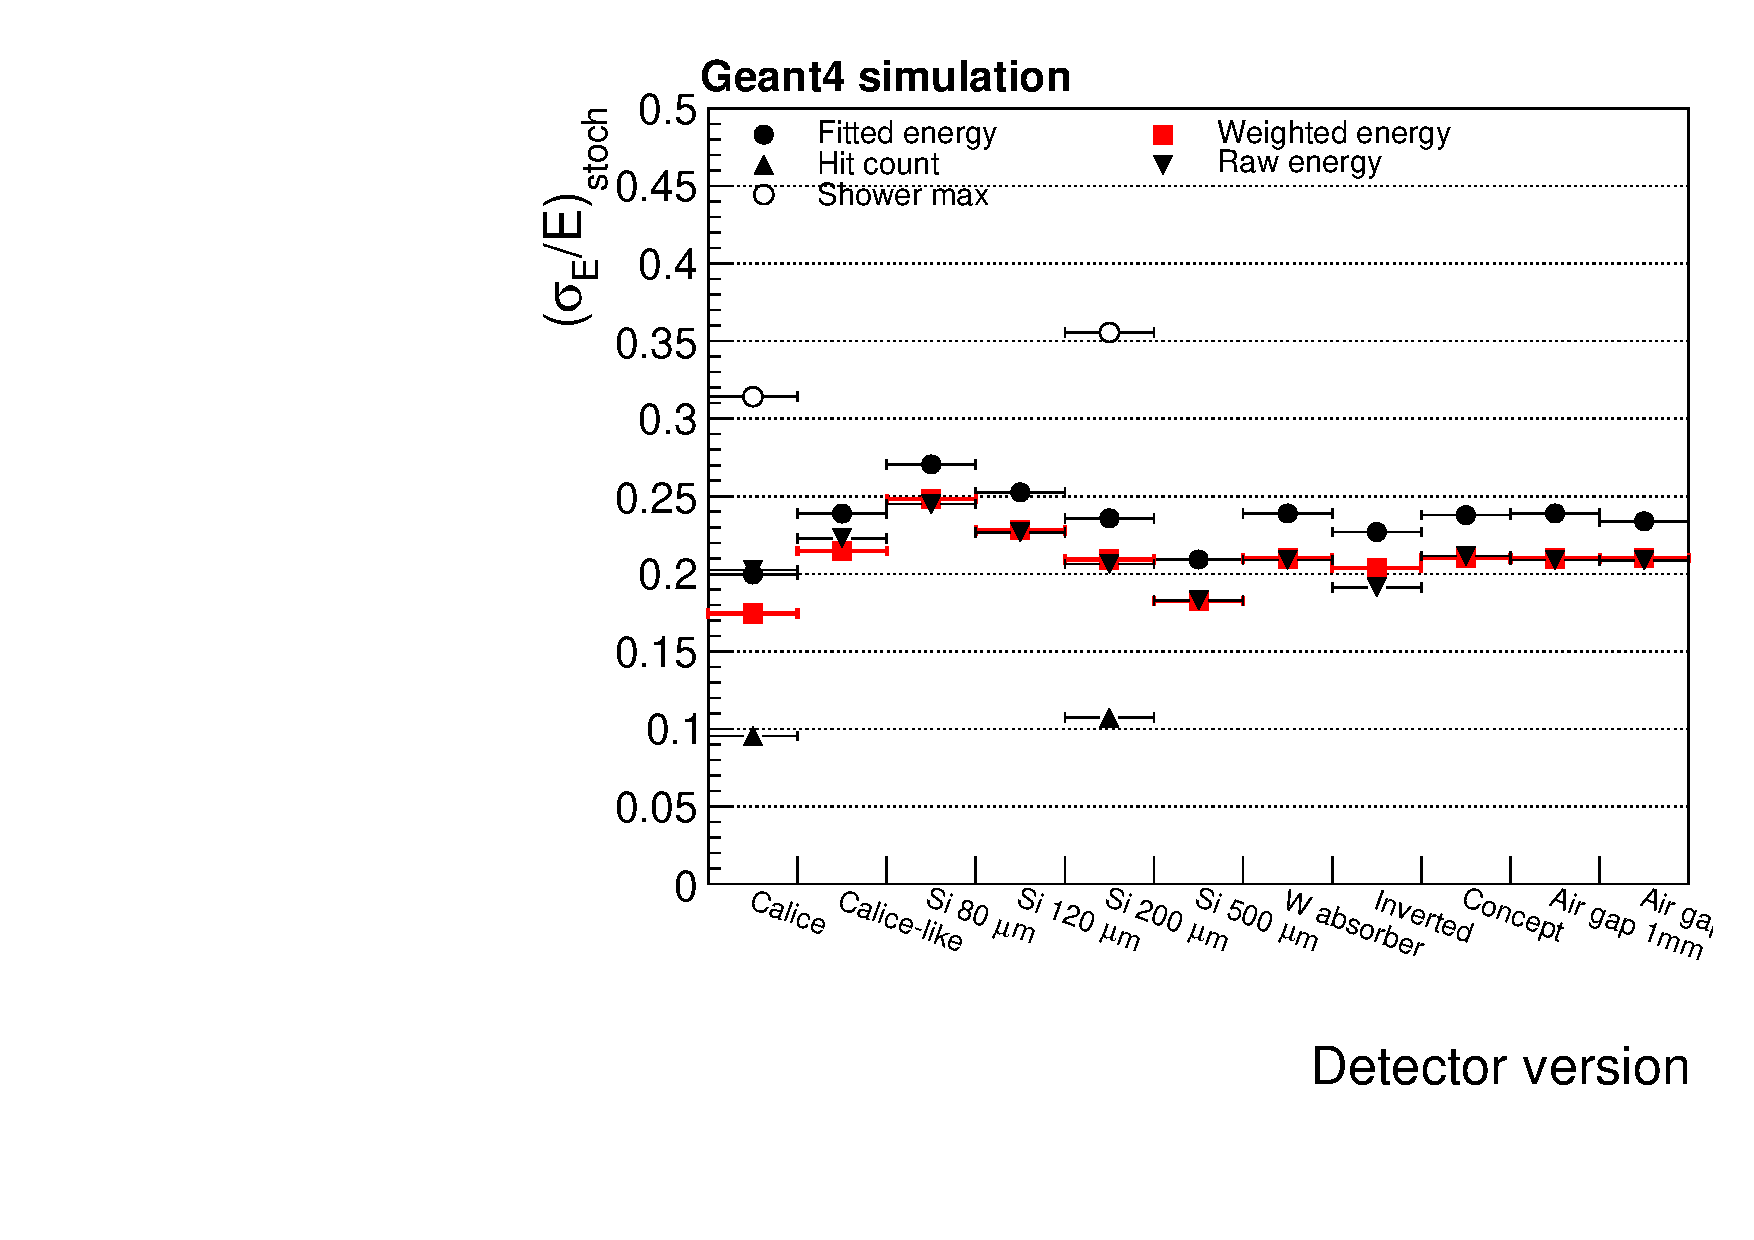
\includegraphics[width=0.75\textwidth]{figures/ResolutionSummary_stochastic}
  \caption{Summary of the fitted resolution curves to different
    setups and using different energy estimators. The constant term
    summary is shown on {\em top} while the stochastic term is
    shown on the {\em bottom}. }
    \label{fig:resol_summary}
  \end{center}
\end{figure}
% AM
\section{Digitisation}
\label{sec:digi}

The digitisation procedure is aimed at converting Geant4 SimHits into
reconstructed hits, i.e. reproducing what the electronics of the real
detector will do given an analogue signal, with a signal and a noise
component, passed through analogue-to-digital (ADC) convertors, with a
zero-suppression threshold applied to reduce the data volume, and
finally the calibration back to an energy.

Minimum ionising particles (MIPs) will deposit energy according to a
Landau distribution, whose maximum probable value can be used to
convert Geant4 energies into other relevant quantities. 

\subsection{The MIP signal}

The energy deposited by 50 GeV muons per $2.5\times 2.5$ mm$^2$ cells
is shown in figure~\ref{fig:muHits}. On the left the number of cells
with energy deposits are shown as a function of the layer, and on the
right the energy deposits for layers which have one and only one hit.

\begin{figure}[h!]
  \begin{center}
    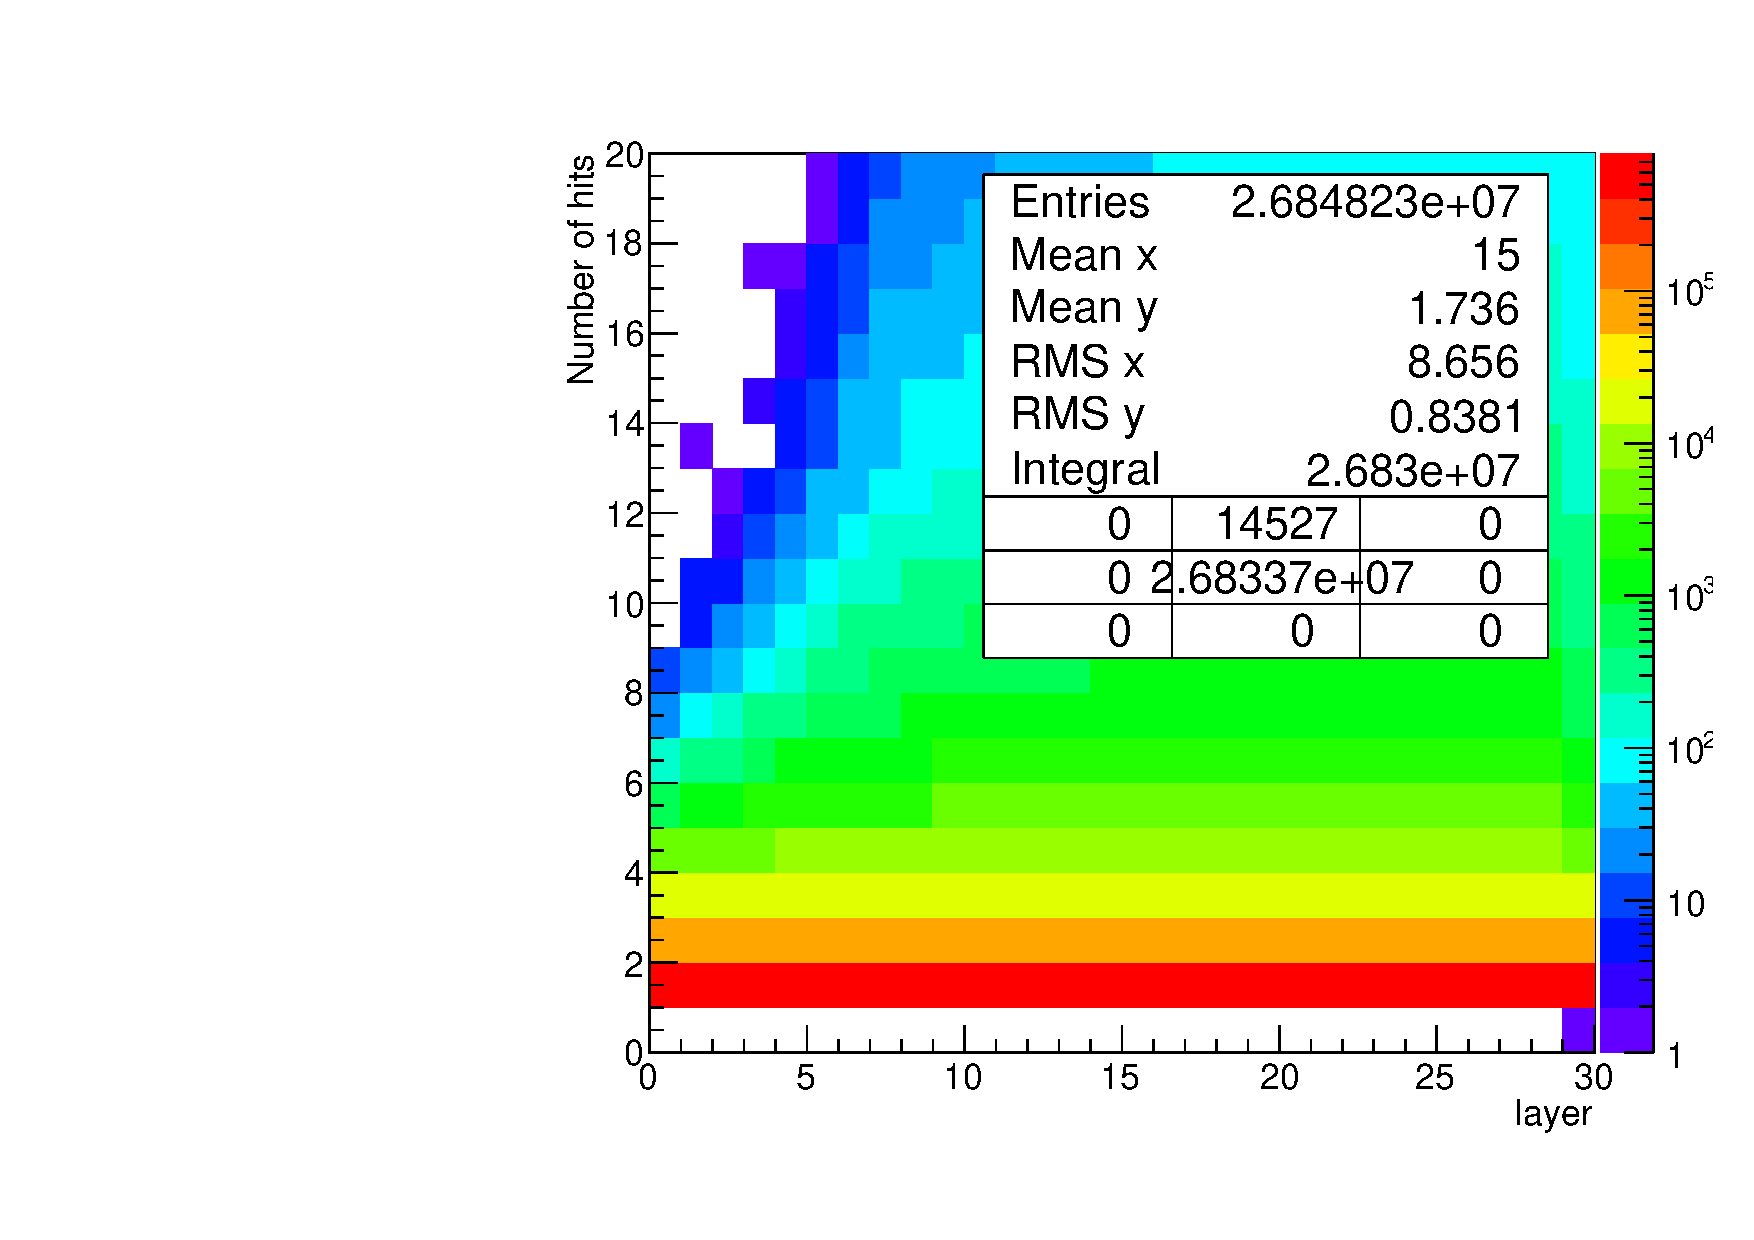
\includegraphics[width=\cmsFigWidth]{figures/mipHits.pdf}
    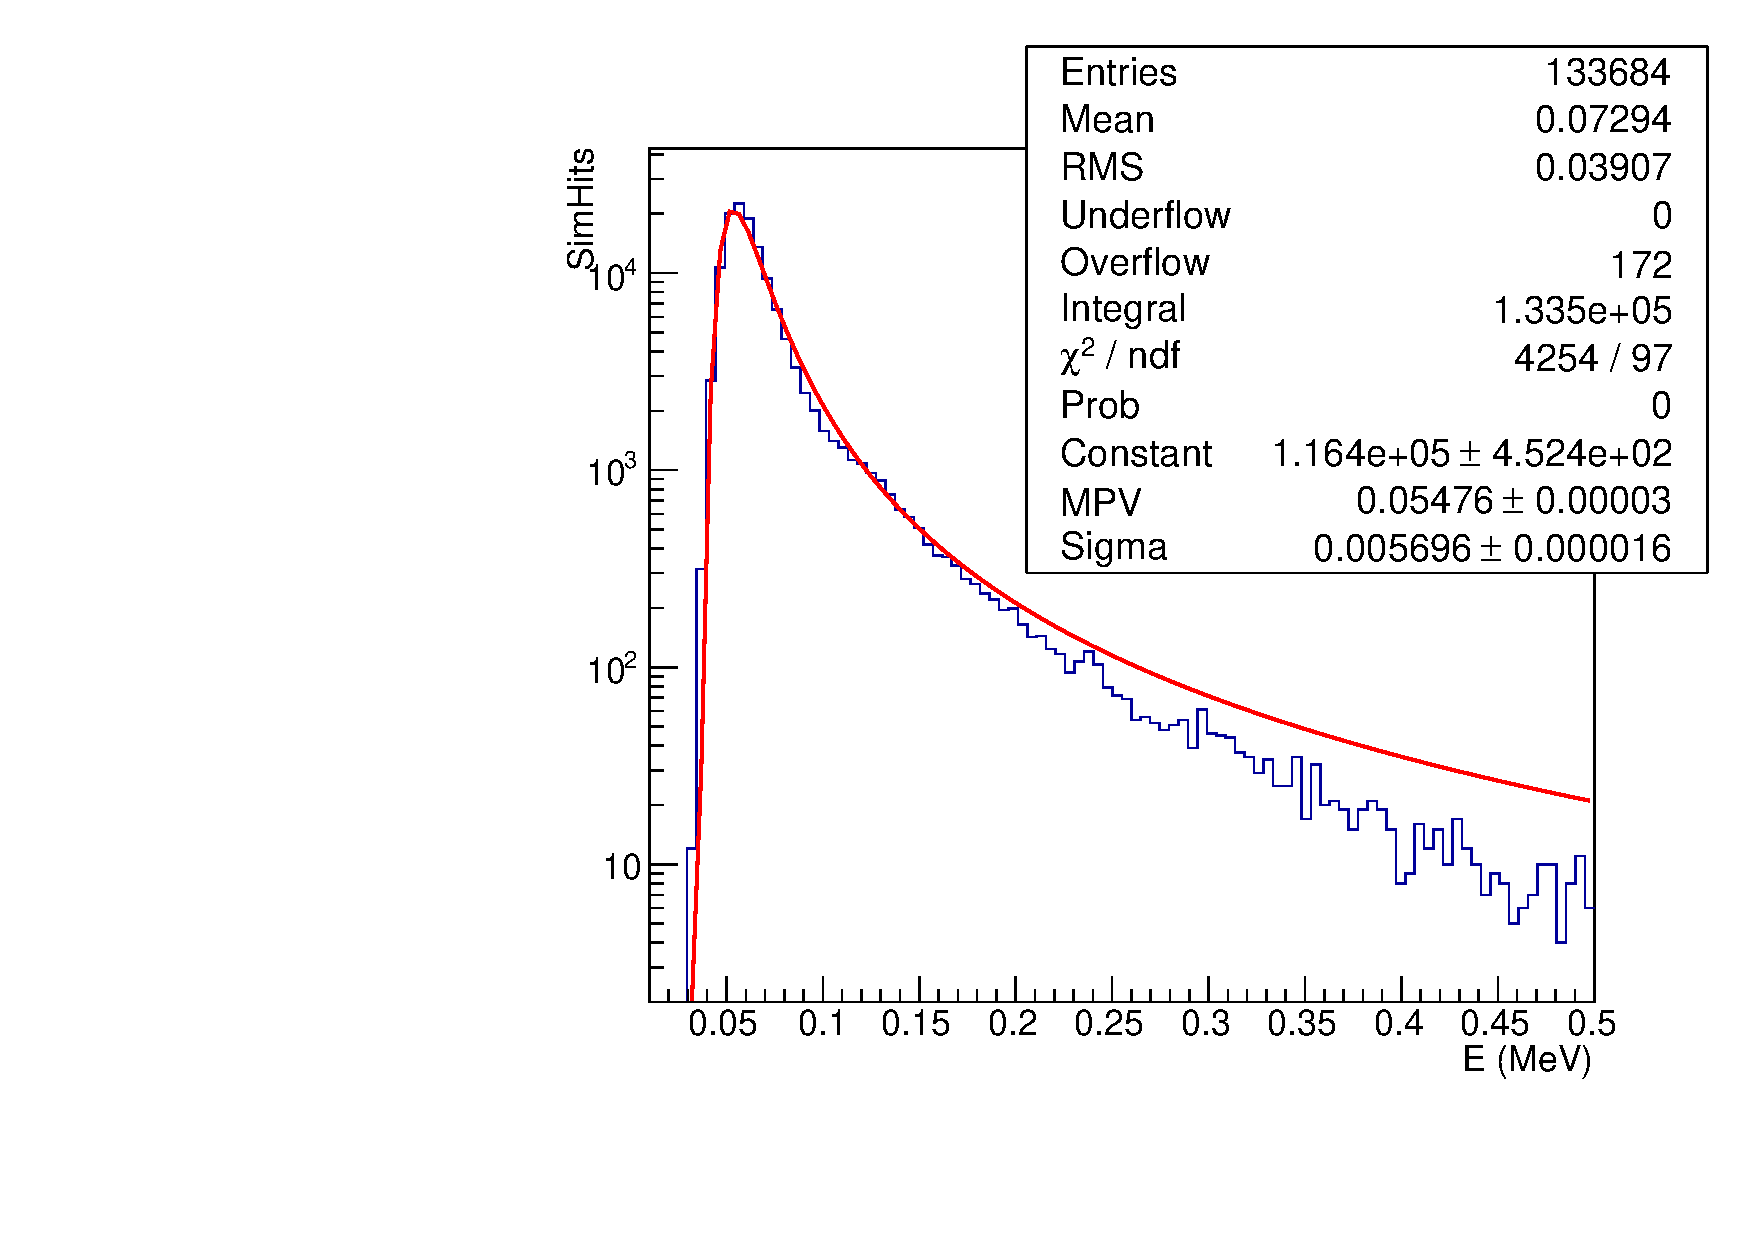
\includegraphics[width=\cmsFigWidth]{figures/mipDepositSel.pdf}
    \caption{}
    \label{fig:muHits}
  \end{center}
\end{figure}

The maximum probable value of the Landau gives the conversion factor
of $$1 \mathrm{MIP} = 0.0545 MeV$$ of energy deposited in Geant4.

\subsection{Electronics calibration and noise}

\subsubsection{MIP to electron conversion}

A MIP will typically create about 75 electron/hole pairs per $\mu$m of
Si. In 200$\mu$m of fully depleted Si, we expect hence about $\simeq
15000$ electrons.

\subsubsection{Dynamic range and MIP to ADC conversion}

The energy deposited by electrons in $1 \times 1$ cm$^2$ Si pads is
shown in figure~\ref{fig:hitE}, on the left for 100 GeV and on the
right for 500 GeV of incoming energy. The dynamic range of the
electronics should hence cover something from below a MIP, in order to
have a calibration peak, and about 1500 MIPs.

\begin{figure}[h!]
  \begin{center}
    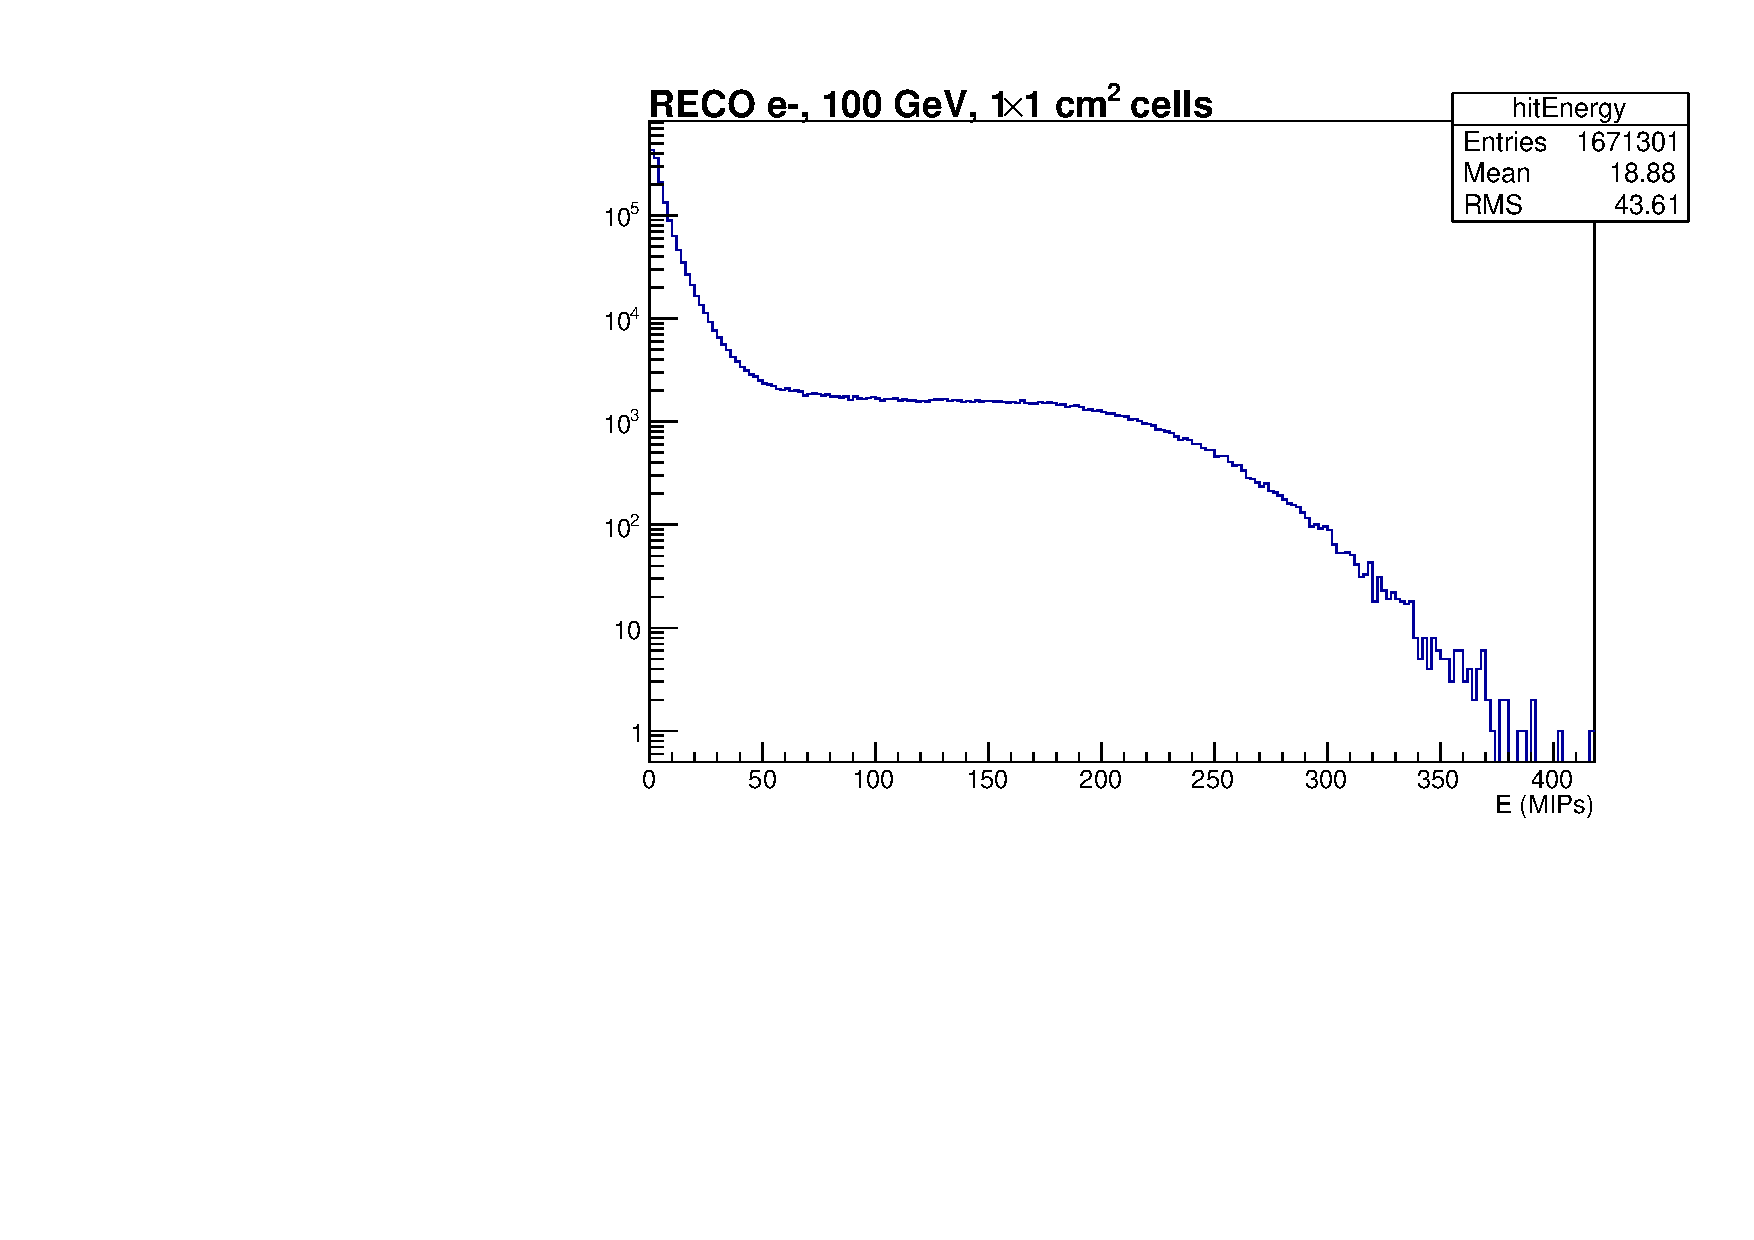
\includegraphics[width=\cmsFigWidth]{figures/HitEnergy_1x1_100GeV.pdf}
    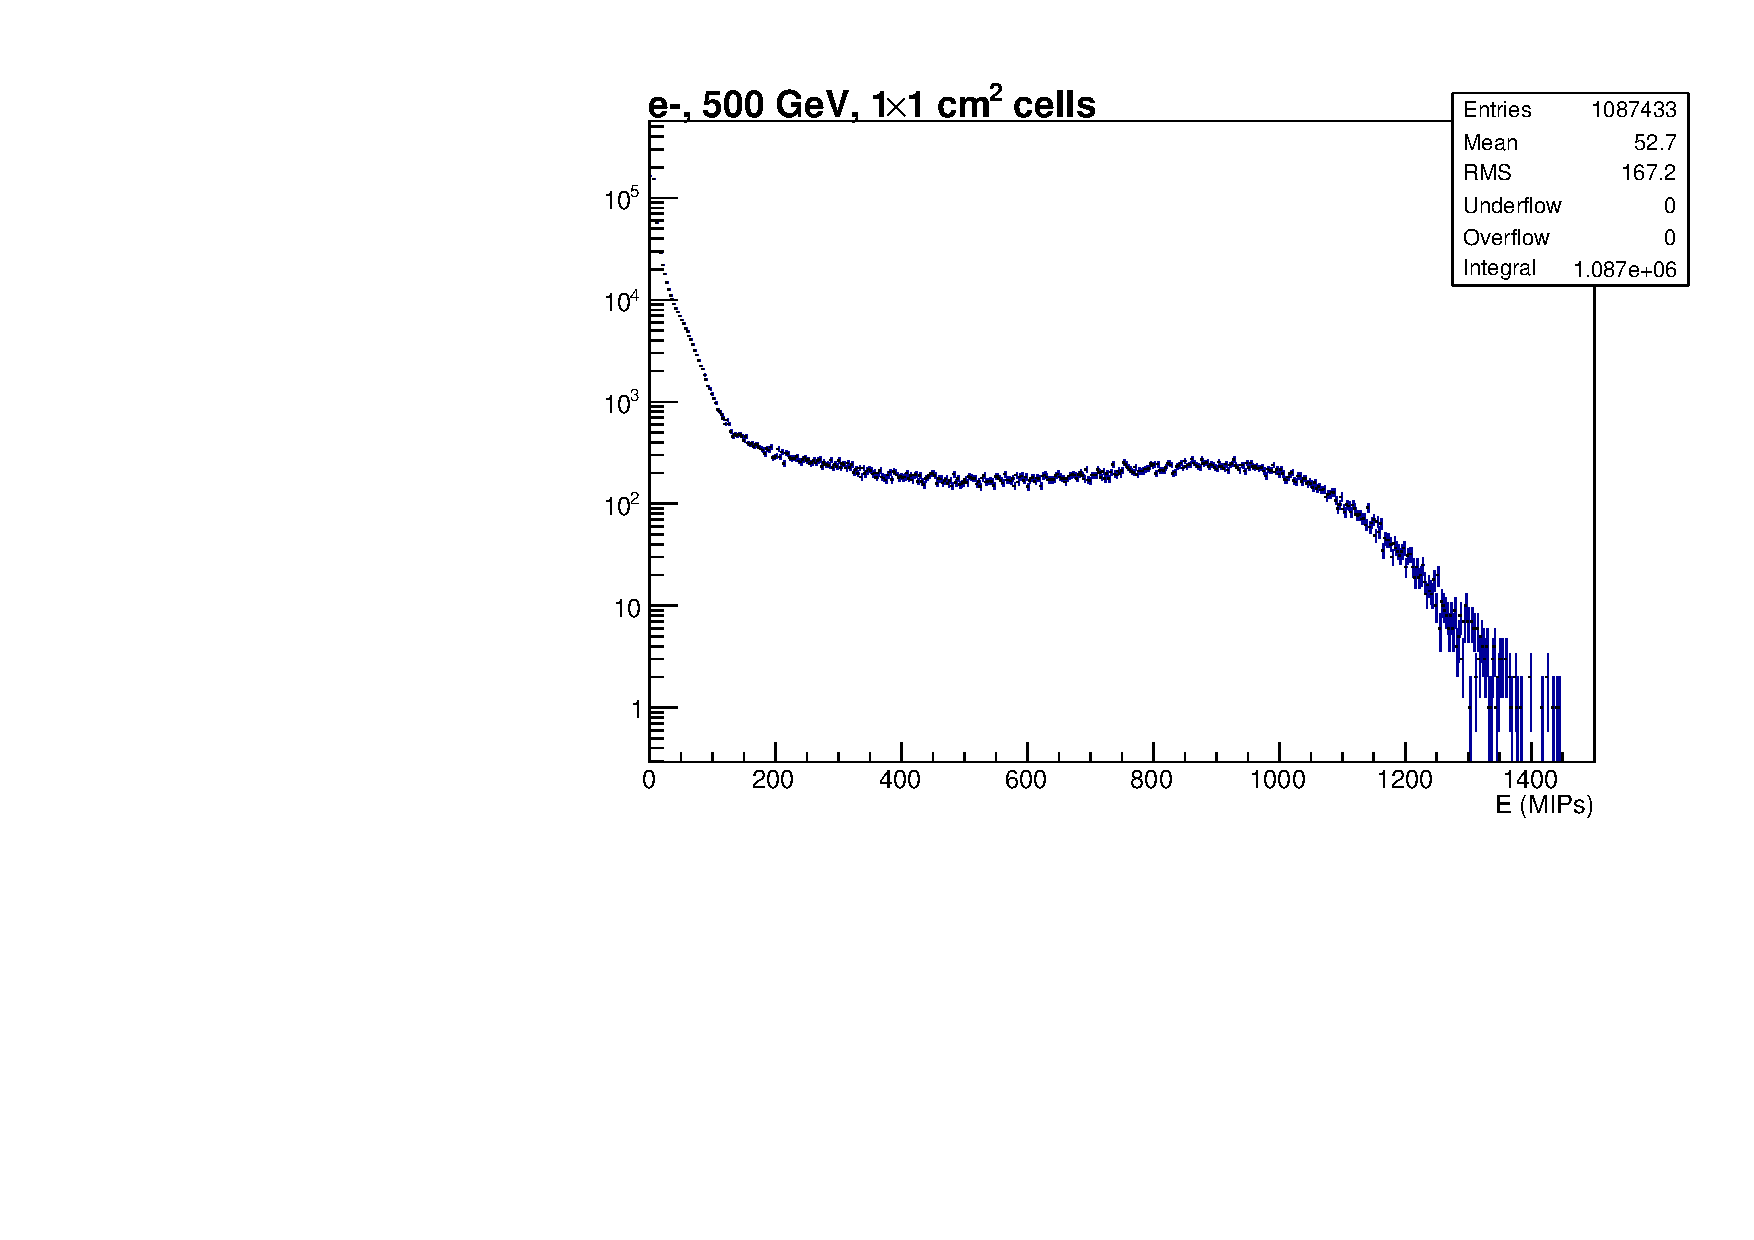
\includegraphics[width=\cmsFigWidth]{figures/HitEnergy_1x1_500GeV.pdf}
    \caption{Energy deposited by electrons per $1 \times 1$ cm$^2$ Si
      pads for 100 GeV (left) and 500 GeV (right) of incoming energy}
    \label{fig:hitE}
  \end{center}
\end{figure}

Three 10-bit ADCs are planned to be used:
\begin{itemize}
\item 10-bit ADC for a range up to 64 MIPs: so 16 ADC counts/MIP or 0.0625 MIP/ADC count.
\item 10-bit ADC for a range up to 1000 MIPs: so 1 ADC counts/MIP.
\item 10-bit ADC for a range up to 10000 MIPs: so 0.1 ADC counts/MIP or 10 MIP/ADC count.
\end{itemize}

The accuracy of the rounding scales as $\frac{x\mathrm{MIPs/ADC
    counts}}{\sqrt{12}}$, so 0.3 MIP for the 1 MIP/ADC count
conversion.

\subsubsection{Noise}

In the CALICE prototype, the signal/noise ratio was measured to be
around 9, so a noise level of about 0.13 MIP. Given this proposal uses
thiner silicon, we can expect a lower signal yield, so comparatively
higher noise. But the noise will decrease with smaller pad sizes, and
with cooling. Note that when using the conversion of 1 MIP / ADC
count, we can expect the noise level to be comparable or lower to the
digitisation accuracy.


\subsubsection{Procedure in software}

The procedure implemented in the standalone simulation is the following:
\begin{itemize}
\item Convert SimHits G4 energy (MeV) to MIPs.
\item Create collection of RecHits with the desired granularity. Baseline: $1 \times 1$ cm$^2$ pads.
\item Add noise in MIPs, included in empty cells.
\item Convert MIPs to ADC counts $\Rightarrow$ DigiHits.
\item Apply threshold: baseline = 5$\times$ noise.
\item Convert ADC counts back to MIPs $\Rightarrow$ RecHits.
\item All parameters are kept configurable for easy scanning.
\end{itemize}

\subsubsection{Impact on the resolution}

\FIXME{Add calibration and resolution curves after digi}
% All
\section{Performances}
\label{sec:perf}

\subsection{Ideal case}

\subsection{After digitisation, varying the parameters}

\subsection{Adding PU}
%
\section{Conclusion}
\label{sec:conclusion}


%% **DO NOT REMOVE BIBLIOGRAPHY**
\bibliography{auto_generated}   % will be created by the tdr script.

%% examples of appendices. **DO NOT PUT \end{document} at the end
%\clearpage
\appendix


%%% DO NOT ADD \end{document}!

